%	\noindent \textbf{RQ2:}\textbf{ Can metrics from code, log and developer dimension help in explaining the stability of logs?}
%	\\\\
%\noindent \textbf{Motivation}

In our preliminary analysis, we find that 35\%-50\% of logs are changed in our subject applications. These log changes affect the log processing tools which run on the studied applications, forcing developers spend more time on maintenance of the log processing tools. By analyzing the factors which can increase the likelihood of a log change, developers of log processing tools can decrease the effort spent on maintenance. 

%understanding which factors can increase the likelihood of a log change, developers of log processing tools can mitigate the effort spent on maintenance by analyzing these factors and avoiding log  

%by performing critical analysis. 


% In this section we construct a random forest model for explaining the likelihood of log changes. We use the random forest model to also identify the most important metrics which explain	whether a log will change in the future. These insights into log 
	
%so that these factors can be taken into account by developers of log processing tools. 

% classifier and ident	ify the important metrics.

% we build a random forest classifier. 


% Hence, there is a need to identify these non-stable logs to simplify the job of developers. It can also benefit log processing tool developers to develop more robust applications making them more stable.

%
%can be extracted from control versions systems by developersthem.  \\


\subsection{Approach}
In this section we construct a random forest classifier for explaining the likelihood of log changes in the studied applications. We then evaluate the performance of our random forest classifier and use it to understand which factors can increase the likelihood of a log change in the studied applications.

We use context and log metrics to train the random forest classifier. Context metrics measure the file context at the time of adding the log. Log metrics measure the details about the added log. We use the Git repository to extract the context metrics and log metrics for the studied applications. 

Table~\ref{tba:Taxonomy} defines each metric collected and the rationale behind our choice of each metric. We use the context metrics as it describes the conditions in which the was added into the application and log metrics provides information about the log added. These metrics also benefit log processing tool developers as they do not need domain knowledge about the application to understand these metrics.\\


%and log metrics because this data can be extracted from the source code repository easily by developers. It also 

%To find the stability of logs in our studied systems, we extract code and log churn metrics from the Git repository and developer metrics from JIRA. We use code churn metrics because prior work has linked logs to development knowledge and issue reports~\cite{IanIcesm}.




%To build prediction models it is necessary to track the changes to logs within the time frame of our study. To achieve this we built a tool which tracks the changes made to each log.  
%
%Since no prior work exists( to our best knowledge ) to predict the stability of logs, we use the code and developer related metrics  to explain the stability of logs. Table ( make table for metrics) explain the different metrics in each category and the rationale for using them. Figure ( make figure explaining process of when log metrics collected and log tracked) shows the process of when metrics are collected and tracking of log. 

%	
%\textbf{Random Forest:} We build random forest to help in predicting the log changes in the revisions of studied systems. A random forest is collection of largely uncorrelated decision trees where they trees combine their results to form a generalized predictor (ref paper). Random forests use bagging strategy (breiman 1996), where the decision trees are constructed using a bootstrap sample dataset. The trees are independent i.e, they do not reply on the earlier trees. In addition to this, random forests split each node using the best among a subset of predictors randomly chosen at that node (breiman 2001). This makes the random forests robust against over-fitting and are more accurate than other tree algorithms (Brieman 2001). 

%\noindent{\textbf{{Model construction}}}

We build random forest classifier~\cite{Albert2008424} to predict whether a log will change in our studied applications. A random forest is a collection of largely uncorrelated decision trees in which the results of all trees are combined to form a generalized predictor. In our classifier, the context and log metrics are the explanatory variables and the dependent class variable is a boolean variable that represents whether the log ever changed or not (i.e., '0' for not changed and '1' for changed).


\begin{figure}
	\centering
	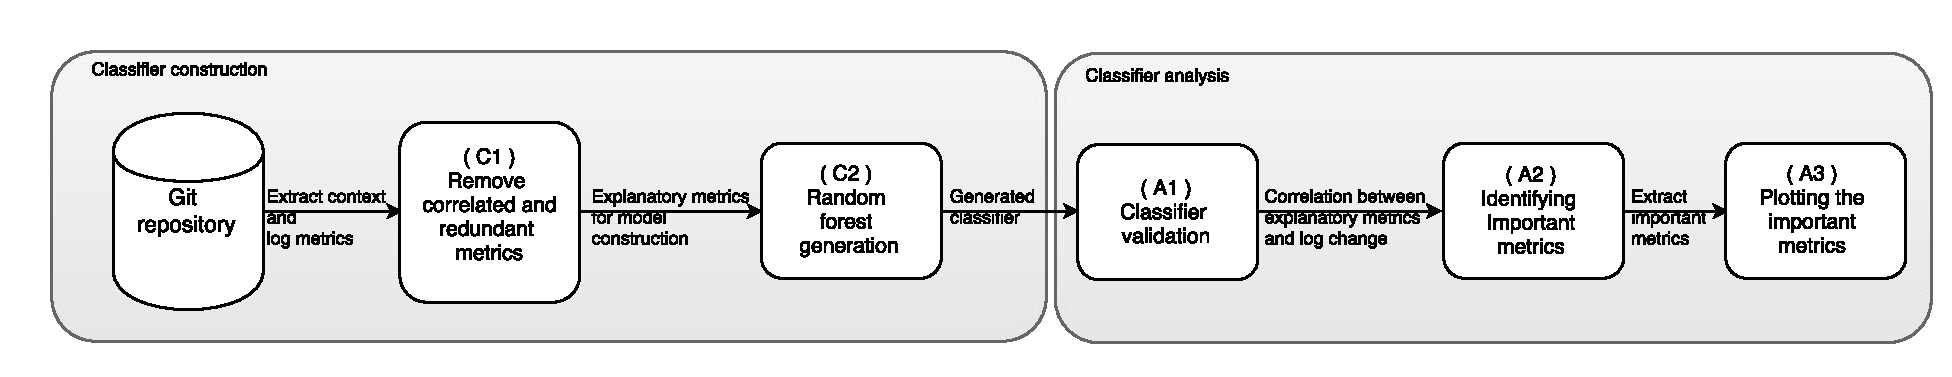
\includegraphics[width=1\columnwidth]{ModelCreationLogGeanology}
	\caption{Overview of random forest classifier construction (C), analysis (A) and flow of data in random forest generation}
	\label{fig:ModelCreationLogGeanology}
\end{figure}  

\begin{table*}
	\centering \protect\caption{The investigated metrics in our clasifier}	
	\label{tba:Taxonomy} %
	\begin{tabular}{c|l|l|>{\raggedright}p{1\columnwidth}}
%		\hline 
\toprule	Dimension  & Metrics  & Values  & Definition (d) -- Rationale (r)\tabularnewline
%		\hline 
		\hline 
		\multirow{12}{*}{Context Metrics} & 

		Log addition & Boolean &
		d: Check if the log is added to the file after creation or it was added when file was created. \tabularnewline
	 &  &  & 
			r: New logs added to a file are more likely to be changed than log previously left untouched in previous commits. 
%			Logs added into a file after creation might be more likely to be changed than the logs added during file creation.
	\tabularnewline 
			
			\cmidrule{2-4} 	&
%		Is readded	 & Boolean (0 -1) &
%		d: Check if the log is readded into a file \tabularnewline
%		\cline{4-4} &  &  &
%		r: Identify the logs which get readded into a file after they are removed. \tabularnewline
%		\cline{2-4} & 		
%		
%		Deleted count & Numerical &
%		d: Number of commits from the time a log is introduced into the file till it is deleted (removed) from the file. \tabularnewline
%		\cline{2-4} &  &  &
%		r: Find out how long it takes before a log is removed from the file. \tabularnewline
%		\cline{2-4} 
	
%		&
%		 New File & Boolean (0 -1) & 
%		d: Check if the log is added in a new file (i.e., newly committed)\tabularnewline
%		\cline{2-4} &  &  & 
%		r: This helps to identify which logs where added later in subsequent commits.\tabularnewline
%		\cline{2-4} 
%		& 
		
		Total revision count & Numerical & d: Total number of commits made to the file before the log is added.
		This value is 0 for logs added in the initial commit but not for logs
		added overtime. \tabularnewline
%		\cline{4-4} 
		&  &  & r: Logs present in a file which is often changed, have higher a likelihood of being changed~\cite{Characterizinglogs}. Hence, the more commits to a file, the higher the likelihood of in that file logs being changed. 
%		chances of logs being changed in a commit as well.
%		Logs present in a file which is changed heavily, have higher chance of being changed.  This helps to find out if the file is changed heavily which can result in log changes~\cite{Characterizinglogs}.
		 \tabularnewline 	\cmidrule{2-4}
		& Code churn in commit & Numerical & d: The code churn of the commit in which a log is added. \tabularnewline
%		\cline{4-4} 
		&  &  & r: Logs added during large code changes like feature addition can be very different from logs added during bug fixes which have lesser code changes.
%		more stable than logs added during bug fixes which have lesser code changes. 
		 \tabularnewline
		\cmidrule{2-4}
		& File ownership  & Numerical  & d: The percentage of the file written by the developer who added the log. \tabularnewline
%		\cline{4-4} 
		 &  &  & r: The owner of the file is more likely to add stable logs than developers who have not edited the file before. 
		 		\tabularnewline		\cmidrule{2-4}
		& Variables declared & Numerical & d: The number of variables which are declared before the log statement in that function.
		\tabularnewline
%		\cline{4-4} 
		&  &  & r: When a large \# of variables are declared, there is higher chance that any of the variables can be changed afterwards. \tabularnewline
	\cmidrule{2-4}
		
		
		& SLOC & Numerical & d: The number of lines of code in the file.\tabularnewline
%		\cline{4-4} 
		&  &  & r: Large files have more functionality and are more prone to changes~\cite{zhang2009investigation}
		and log changes~\cite{Characterizinglogs,EMSEIAN}.
		 \tabularnewline
		 \cmidrule{2-4}
		& Developer experience & Numerical & d: The number of commits the developer has made prior to this commit. \tabularnewline
%		\cline{4-4} 
		&  &  & r: More experienced developers may add more stable logs than a new developer who has little understanding of the application. 
	 \tabularnewline
%		Research has shown that experienced developers might take up more
%		complex issues~\cite{rahman2011ownership} and therefore may leverage
%		logs more~\cite{EMSEIAN}.

%		\cline{2-4} 	
\cmidrule{2-4}	 
%		\hline
		\cmidrule{1-4} 
		\multirow{22}{*}{Log Metrics} & Log context & Categorical & d: The block in which a log is added i.e., \emph{if, if-else,
		try-catch, exception, throw, new function}.\tabularnewline
%		\cline{4-4} 
		&  &  & r: Prior research finds that logs are mostly used in assertion checks,
		logical branching and return value checking~\cite{Fu1}. Logs used in logical branching and assertion checks, i.e., if-else blocks, may be very different from the logs in try-catch, exception blocks. \tabularnewline
\cmidrule{2-4}
		 &
	Is re-added	 & Boolean &
		d: Check if the log is re-added into a file. \tabularnewline
%	\cline{4-4}
	 &  &  &
	r: Logs which are added, removed and re-added into a file suggest that developers are unsure of the purpose of the log making them very unstable and prone to changes.  \tabularnewline
\cmidrule{2-4}
%	& 	
%		Log change type	 & Categorical &
%		d: Check the type of log change the log has undergone before, i.e., relocation, text-variable change, level change. \tabularnewline
%		\cline{4-4}
%		 &  &  &
%		r: Changes to log text, variable and verbosity level can make logs more unstable than relocation changes.    
%		\tabularnewline
%\cmidrule{2-4}
%		
		& Log variable count & Numerical & d: Number of logged variables.\tabularnewline
%		\cline{4-4} 
		&  &  & r: Over 62\% of log changes add new variables~\cite{Characterizinglogs}.
		Hence, fewer variables in the initial log statement might result in
		addition of new variables later. \tabularnewline
\cmidrule{2-4}
		& Log density & Numerical & d: Ratio of the number of log lines to the source code lines in the file.\tabularnewline
%		\cline{4-4} 
		&  &  & r: Files which are well logged (i.e., higher log density) may not need additional logs and the logs are less likely to be changed.
		\tabularnewline
\cmidrule{2-4}
		& Log level & Categorical & d: The log level (verbosity) of the added log, i.e., \emph{info,error, warn, debug, trace} and \emph{trace}.\tabularnewline
%		\cline{4-4} 
		&  &  & r: Research has shown that developers spend significant amount of time in adjusting the verbosity of logs~\cite{Characterizinglogs}. Hence, higher level logs such as \emph{warn} and \emph{error} might be more thought out than default level \emph{info} logs. \tabularnewline
\cmidrule{2-4}
		& Log text count & Numerical & d: Number of text phrases logged. We count all text present between a pair of quotes as one phrase.\tabularnewline
%		\cline{4-4} 
		&  &  & r: Over 45\% of logs have modifications to static context~\cite{Characterizinglogs}.
		Logs with fewer phrases might be subject to changes later to provide a
		better explanation.\tabularnewline
\cmidrule{2-4} &
		Log churn in commit	 & Numerical &
		d: The number of logging statements changed in the commit. \tabularnewline
		\cline{4-4}
		 &  &  &
		r:  Logging statements can be added as part of specific change or part of bigger change. 
		\tabularnewline
		\cmidrule{1-4}
%		\cline{2-4} 	
%		& Resolution time & Numerical & d: The time it takes for the issue to get fixed. It is defined as
%		the time it takes since an issue is opened until closed. \tabularnewline
%		\cline{2-4} 
%		&  &  & r: More resolution time might suggest a more complex fix with more
%		log churn. \tabularnewline
%		\cline{2-4} 
%		& Number of developers involved & Numerical & d: Total number of unique developers who contribute to the file.\tabularnewline
%		\cline{2-4} 
%		&  &  & r: Components with many unique authors likely lack strong ownership, which in turn may lead to more defects~\cite{mcintosh2014impact}
%		and change logs~\cite{EMSEIAN}. \tabularnewline
%		\cline{2-4} 
%		& Number of comments & Numerical & d: Total number of discussion posts on the issue. \tabularnewline
%		\cline{2-4} 
%		&  &  & r: Number of comments is correlated to the resolution time of issue
%		reports~\cite{giger2010predicting}. More comments may also indicate
%		the issue is more complex resulting in more code churn and log changes. \tabularnewline
%		\cline{2-4} 

%		& Issue type  & Categorical & d: Identify the type of issue, i.e., `Bug', `Improvement', `Task',
%		`New Feature', `Sub-Task', `Test'. \tabularnewline
%		\cline{2-4} 
%		&  &  & r: Some issue types might have higher code churn than others (example:
%		Bug and New features might have more code churn when compared to Sub-Tasks)
%		and are committed faster.\tabularnewline
%		\cline{2-4} 
%		& Priority type & Categorical & d: Identify the priority of the issue i.e., `Critical', `Blocker',
%		`Major', `Minor' and `Trivial'\tabularnewline
%		\cline{2-4} 
%		&  &  & r: Research has shown that priority of issue affects resolution time
%		of bug fixes~\cite{MarkFixTime}. A Higher priority indicates the
%		issue will be fixed faster with log changes. \tabularnewline
%		\cline{2-4} 

%		\hline 
	\end{tabular}\protect
\end{table*}



Figure~\ref{fig:ModelCreationLogGeanology} provides an overview of the construction steps (C1 to C3) for building a random forest classifier and steps (A1 and A2) provides an analysis of the results. We use the statistical tool R to model our data using the \emph{RandomForest} package.\\

\subsection*{Step C1 - Removing Correlated Metrics}
%\textbf{\textsl{(C1 - Correlation analysis) }}

Correlation analysis is necessary to remove the highly correlated metrics from our dataset~\cite{correlationBook}. Correlated metrics can severely impact the calculation of importance in the random forest classifier, as small changes to one correlated metric can affect the values of the other correlated metrics, causing large changes on dependent class variable. 

%Collinearity between metrics can affect the performance of a model because small changes in one metric can affect the values of other metrics causing large changes on the dependent class variable. 

We use Spearman rank correlation~\cite{spearmanbook} to find correlated metrics in our data. Spearman rank correlation assesses how well two metrics can be described by a monotonic function. We use Spearman rank correlation instead of Pearson~\cite{pearsonbook} because Spearman is resilient to data that is not normally distributed. We use the function \emph{varclus} in R to perform the correlation analysis.

Figure~\ref{fig:SpearmanActiveMQ} shows the hierarchically clustered Spearman $\rho $ values in the ActiveMQ project. The solid horizontal lines indicate the correlation value of the two metrics that are connected by the vertical branches that descend from it.  We include one metric from the sub-hierarchies which have correlation $|\rho| > 0.7 $. The gray line indicates our cutoff value ($ | \rho | $ = 0.7). We use cutoff value of ($ | \rho | $ = 0.7) as used by prior research~\cite{ShaneOLS} to remove the correlated metrics before building our model. We find that \emph{total revision count} is highly correlated with \emph{code and log churn in commit}, because a file with more commits has higher chance of having a large commit with log changes, than a file with fewer commits. We exclude \emph{total revision count} and \emph{log churn in commit} and retain \emph{code churn in commit} as it is a simpler metric to compute. \\





\begin{figure}
	\centering
	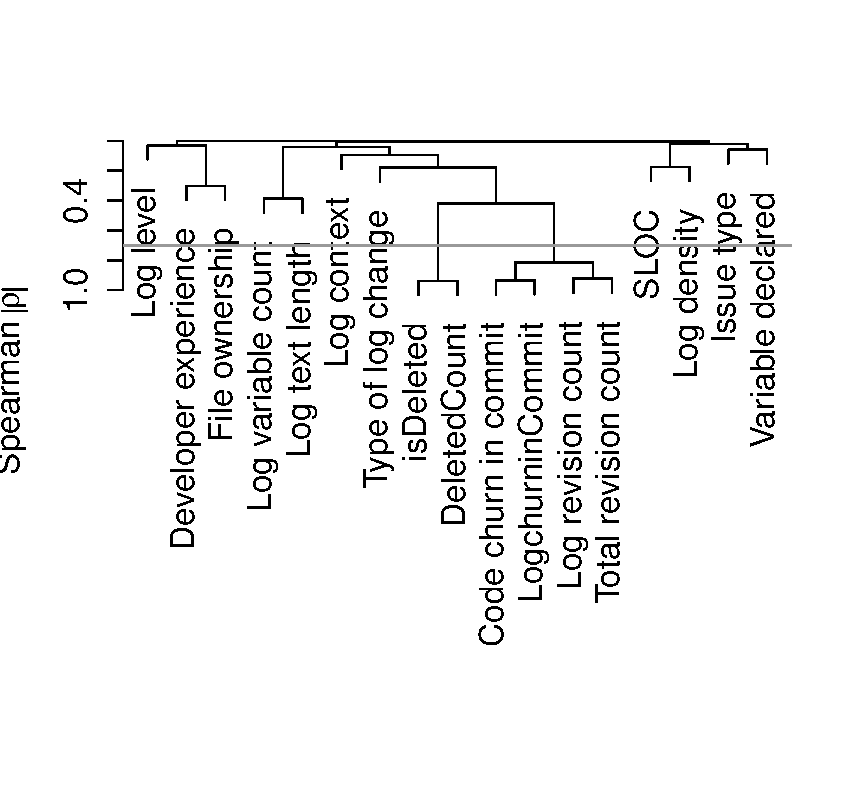
\includegraphics[height=0.8\columnwidth,width=0.9\columnwidth]{SpearmanActiveMQ}
 \vspace*{-1cm}	\caption{Hierarchical clustering of variables according to Spearman’s $\rho$ in ActiveMQ}
	\label{fig:SpearmanActiveMQ}
\end{figure}


\subsection*{Step C2 - Random Forest Generation}
%\textbf{\noindent\textsl{(C2 - Random forest generation)}}

After we eliminate the correlated metrics from our datasets, we construct the random forest model. Random forest is a black-box ensemble classifier, which operates by constructing a multitude of decision trees on the training set and uses this to classify the testing set. From a training set of $m$ logs a random sample of \emph{n} components is selected with replacement~\cite{ShaneOLS} and using the \emph{randomForest} function from the \emph{randomForest} package in R, a random forest model is generated. 

%Figure~\ref{fig:BootRF} explains the construction of the random forest classifier, where 

%From the sampled selection, many classification trees are grown without pruning. Each classification tree gives a vote, i.e., \emph{true} if log is changed and \emph{false} if not. The random forest chooses the class with most number of votes over all the trees in the forest. This strategy helps to make the random forests more robust against over-fitting~\cite{breiman1996bagging}.

%and the steps are explained below.
%\begin{figure}
%	\centering
%	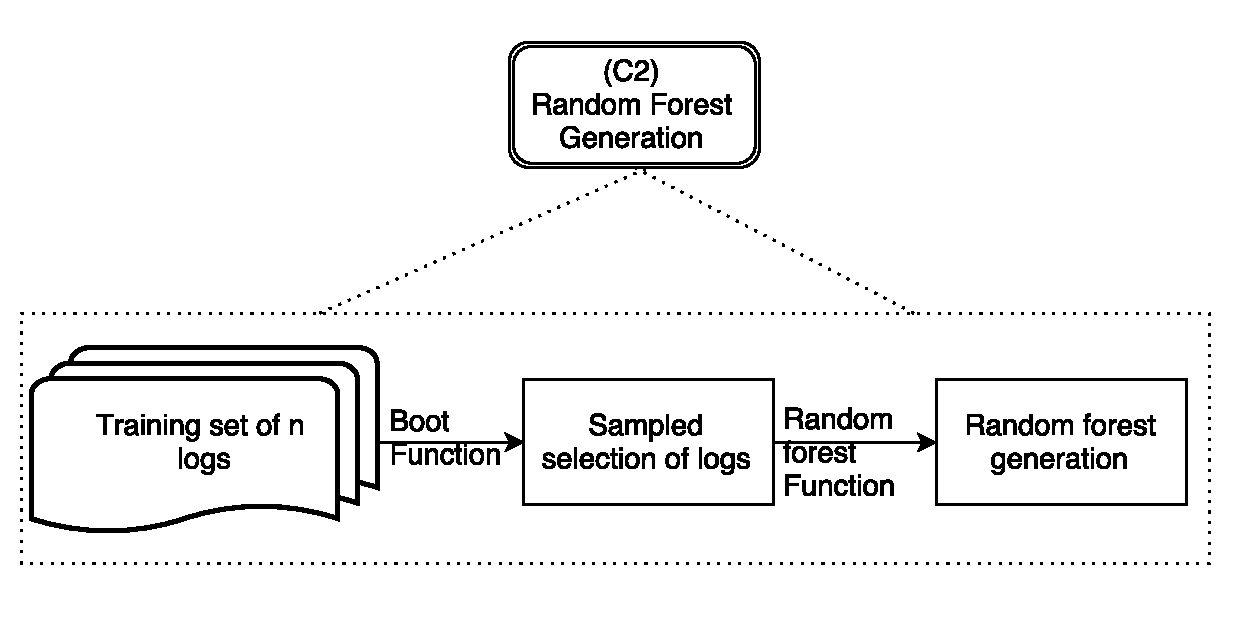
\includegraphics[height=.5\columnwidth,width=1\columnwidth]{BootRandomForest}
%	\caption{Overview of random forest generation in C2}
%	\label{fig:BootRF}
%\end{figure}


%Given a dataset of \textsl{m} logs for training, $ D = \{ (X_{1}Y_{1}),...,(X_{m}Y_{m}) \} $ where $X_{i, i = 1...m}$, is a vector of descriptors (i.e., $X$ are the metrics which are left after correlation analysis ) and $Y_{i}$ is the flag which indicates whether a log is changed or not.

%\begin{enumerate}
%\item From the training set of \textsl{m} logs, a random sample of \emph{n} components is selected with replacement (i.e., bootstrap sample)~\cite{ShaneOLS}.
%
%We use the \emph{boot} function from the \emph{boot} package in R to generate bootstrap samples. The boot function generates a set of random indices, with replacement from the integers 1:\emph{n}.
%
%\item From the sampled selection, many classification trees are grown without pruning. Each classification tree gives a vote, i.e., \emph{true} if log is changed and \emph{false} if not. The random forest chooses the class with most number of votes over all the trees in the forest. This strategy helps to make the random forests more robust against over-fitting~\cite{breiman1996bagging}.
%
% We use the \emph{randomForest} function from the \emph{randomForest} package in R to generate the random forest model. 
%
%
%\item The above steps are repeated until \textsl{M} such models are grown.
%\item Predict new data by aggregating the prediction of the $M$ models generated.
%\end{enumerate}  

\begin{table}[t]
	\centering
		\caption{Confusion Matrix}
		\label{tba:confusion}
	\begin{tabular}{|ll|l|l|}
		\cline{1-4}
		&                 & \multicolumn{2}{c|}{Predicted}            \\ \cline{3-4} 
		&                 & Log changed         & Log not changed     \\ \hline
		\multicolumn{1}{|c|}{\multirow{2}{*}{Actual}} & Log change      & True positive (TP)  & False negative (FN) \\ \cline{2-2} 
		\multicolumn{1}{|c|}{}                        & Log not changed & False positive (FP) & True negative (TN)  \\ \hline
	\end{tabular}
		

\end{table}

%\begin{table}[t]
%
%	\begin{tabular}{|>{\raggedright}p{0.1\columnwidth}>{\raggedright}p{0.2\columnwidth}|l>{\raggedright}p{0.2\columnwidth}|}
%		\hline 
%		\multicolumn{1}{|>{\raggedright}p{0.03\columnwidth}}{\multirow{2}{0.03\columnwidth}{}} &  & \multicolumn{2}{c|}{Predicted}\tabularnewline
%		&  & Log has changed & Log has not-changed\tabularnewline
%		\hline 
%		\multirow{2}{0.03\columnwidth}{Actual} & Log has changed  & TP (True Positive)  & FN (False Negative ) \tabularnewline
%		& Log has not-Changed  & FP (False Positive )  & TN (True Negative) \tabularnewline
%		\hline 
%	\end{tabular}\protect
%	
%	
%
%\end{table}
\subsection*{Step A1 - Model validation}
%\textbf{\noindent \textsl{(C3 - Model evaluation)}}

After we build the random forest model, we evaluate the performance of our model using precision, recall, F-measure, AUC and Brier Score. These measures are functions of the confusion matrix as shown in Table~\ref{tba:confusion} and are explained below.

\textsl{Precision (P)} measures the correctness of our model in predicting which log will change in the future. Precision is defined as the number of logs which were accurately predicted as changed over all logs predicted to have changed as explained in Equation~\ref{f:precision}.   \\
	 \begin{equation}
 P =  \dfrac{TP}{TP + FP } 
 \label{f:precision}
	 \end{equation}	
	 
\textsl{Recall (R)} measures the completeness of our model. A model is said to be complete if the model can correctly classify all the logs which will get changed in our dataset. Recall is defined as the number of logs which were accurately predicted as changed over all logs which actually change as explained in Equation~\ref{f:recall}.
	 \begin{equation}
	 R =  \dfrac{TP}{TP + FN } 
	 \label{f:recall}
	 \end{equation}	
	 
\textsl{F-Measure} is the harmonic mean of precision and recall, combining the inversely related measure into a single descriptive statistic as shown in Equation~\ref{f:Fmeasure}~\cite{F-Measure}.
	 \begin{equation}
	 F =  \dfrac{2 \times P \times R}{P + R } 
	 \label{f:Fmeasure}
	 \end{equation}	

\textsl{Area Under Curve (AUC)} is used to measure the overall ability of the model to classify changed and unchanged logs. The value of AUC ranges between 0.5 (worst) for random guessing and 1 (best) where 1 means that our model can correctly classify every log as changed or unchanged. 



%a measure of the accuracy of the predictions in our model~\cite{wilks2011statistical}. It explains how well the model performs compared to random guessing i.e.,  a perfect classifier  will have Brier score of 0 and perfect misfit classifier will have Brier score of 1 (predicts probability of log change when log not changed). This means the lower the Brier score value, the better our random forest classifier.
	 
\textsl{Brier score (BS)} is a measure of the accuracy of the predictions in our model~\cite{wilks2011statistical}. Brier score explains how well the model performs compared to random guessing as explained in Equation~\ref{f:BS}, where $P_{t}$ is the probability of log change, $O_{t}$ is the actual log being changed or not. A perfect classifier will have a Brier score of 0, a perfect misfit classifier will have a Brier score of 1 (predicts probability of log change when log is not changed) and for random guessing Brier score reaches the value of 0.25. This means lower the Brier score value, the better our random forest classifier.

% This means lower the Brier score value, the  accuracy of random forest classifier and Brier score reaches the value 0.25 for random guessing. 

% The lower the Brier score value, the better our random forest classifier and reaches 0.25
%As the Brier score measure the total difference between the event and the forecast probability of the event, 
 
%The most common formulation of Brier Score is shown in Equation~\ref{f:BS}, where $f_{t}$ is the probability that was predicted, $o_{t}$ is the actual outcome of the event at the instance $t$ (0 if log is not changed and 1 if it is changed), and $N$ is the number of forecasting instances. 

%If the predicted value is 70\% and the log is changed, the Brier Score is 0.09 (lower the Brier score, the more likely the event will occur). It reaches 0.25 

	 \begin{equation}
	 BS =  (P_{t} - O_{t} )^{2} 
	 \label{f:BS}
	 \end{equation}	

The performance measures described previously, may overestimate the performance of the classifier due to over fitting. To account for the overfitting in our models, we use the \textsl{optimism} measure, as used by prior research~\cite{ShaneOLS}. The \textsl{optimism} of the performance measures are calculated as follows:
\begin{enumerate}
	\item From the original dataset with \textsl{m} records, we select a bootstrap sample with \textsl{n} records with replacement.
	\item Build random forest as described in (C2) using the bootstrap sample.
	\item Apply the classifier model built from the bootstrap sample on both the bootstrap and original data sample, calculating precision, recall, F-measure and Brier score for both data samples.
	\item Calculate the \textsl{optimism} by subtracting the performance measures of the bootstrap sample from the original sample. 	
\end{enumerate}

	The above process is repeated 1,000 times and the average (mean) \textsl{optimism} is calculated. Finally, we calculate \textsl{optimism-reduced} performance measures for precision, recall, F-measure, AUC and Brier score by subtracting the averaged optimism of each measure, from their corresponding original measure.  The smaller the optimism values, less of an overfit the original classifier is.
	\\

\begin{figure}[tb]
	
	\centering
	\subfloat{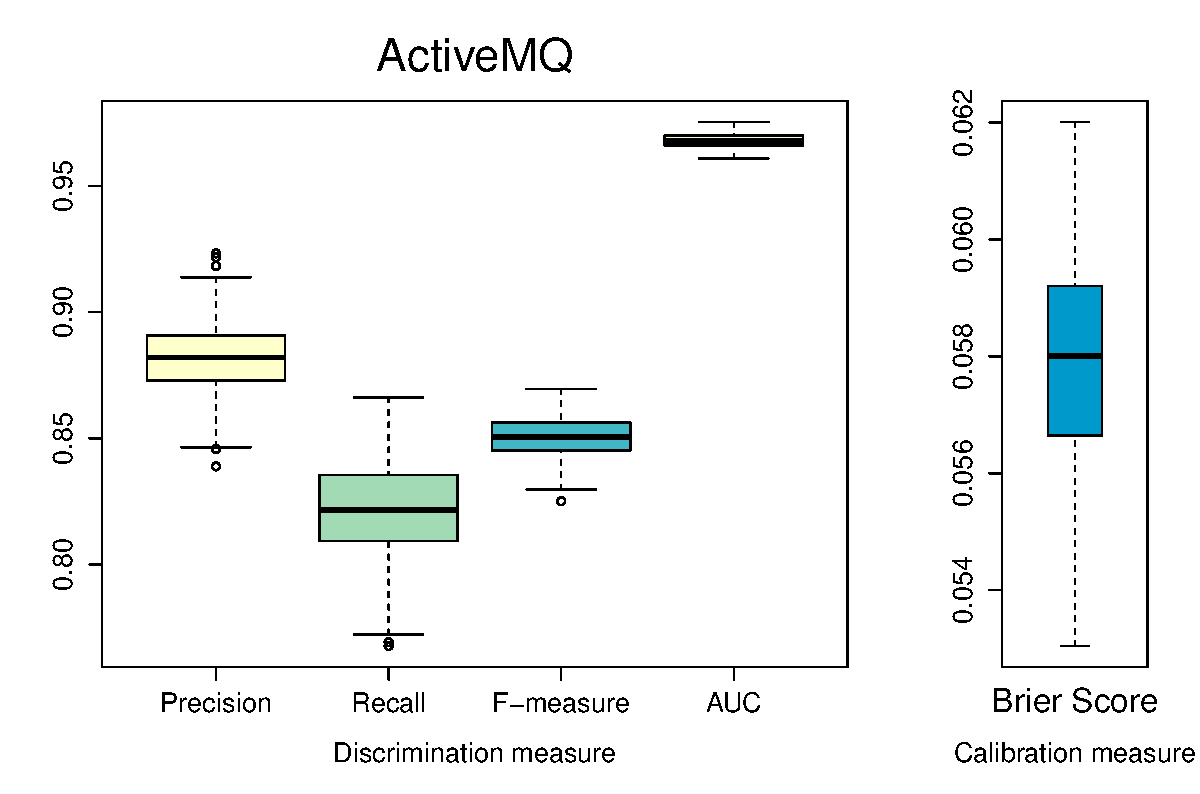
\includegraphics[width=0.69\columnwidth]{ARBox}\label{fig:f41}}
	\hfill
	\centering
	\subfloat{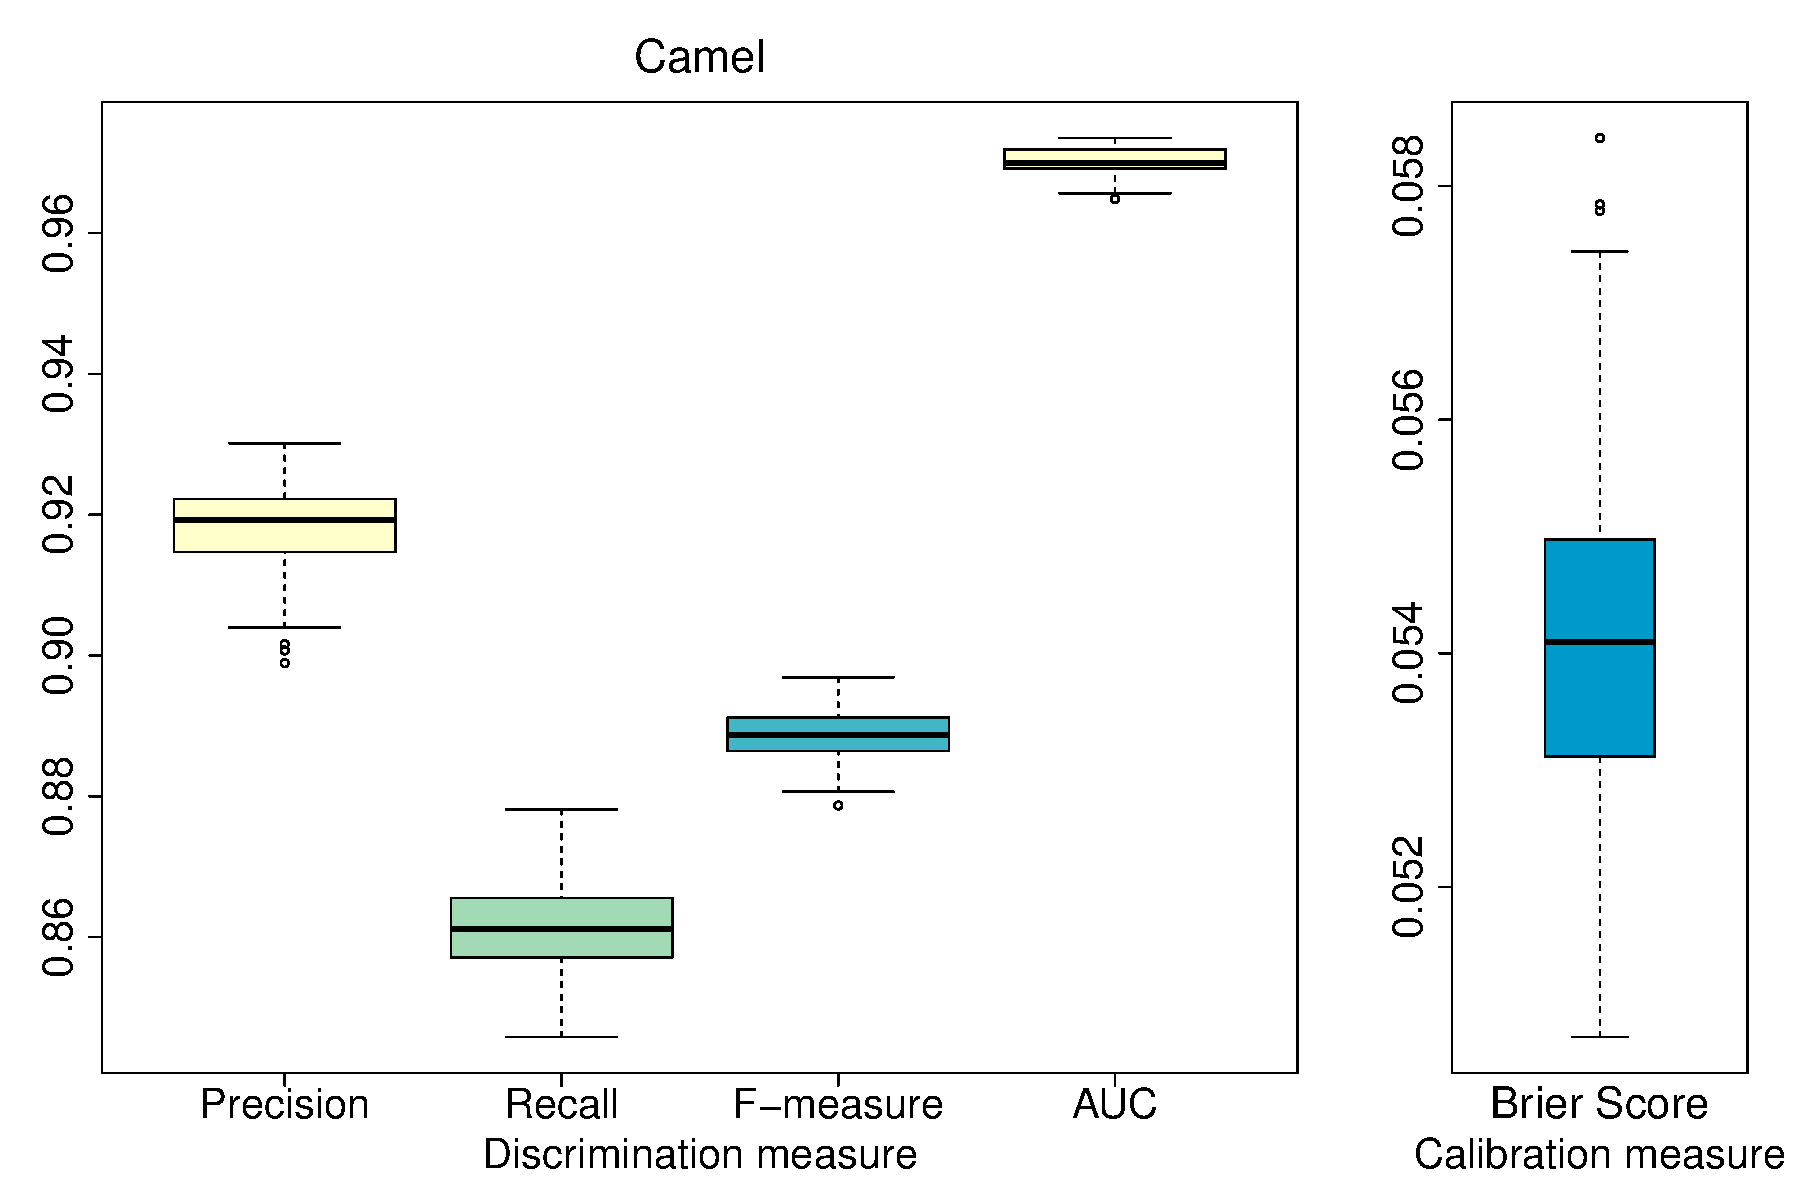
\includegraphics[width=0.69\columnwidth]{CRBox} }
	\hfill
	\centering
	\subfloat{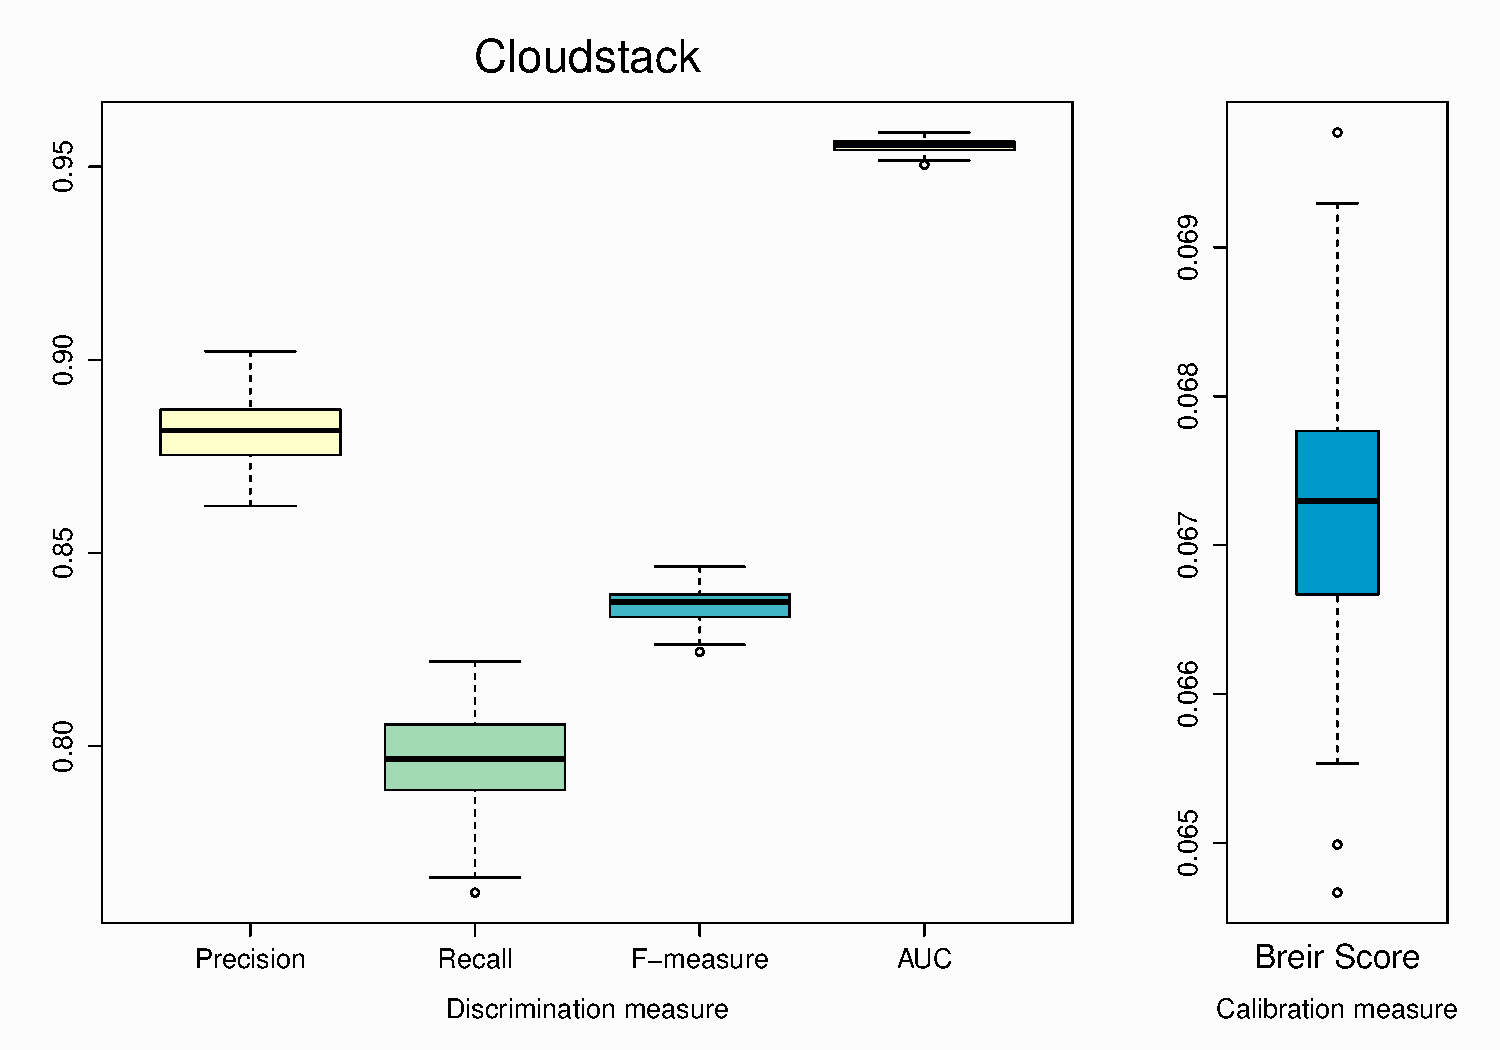
\includegraphics[width=0.69\columnwidth]{CloRBox}
		\label{fig:f42}}
	\hfill
	\centering
	\subfloat{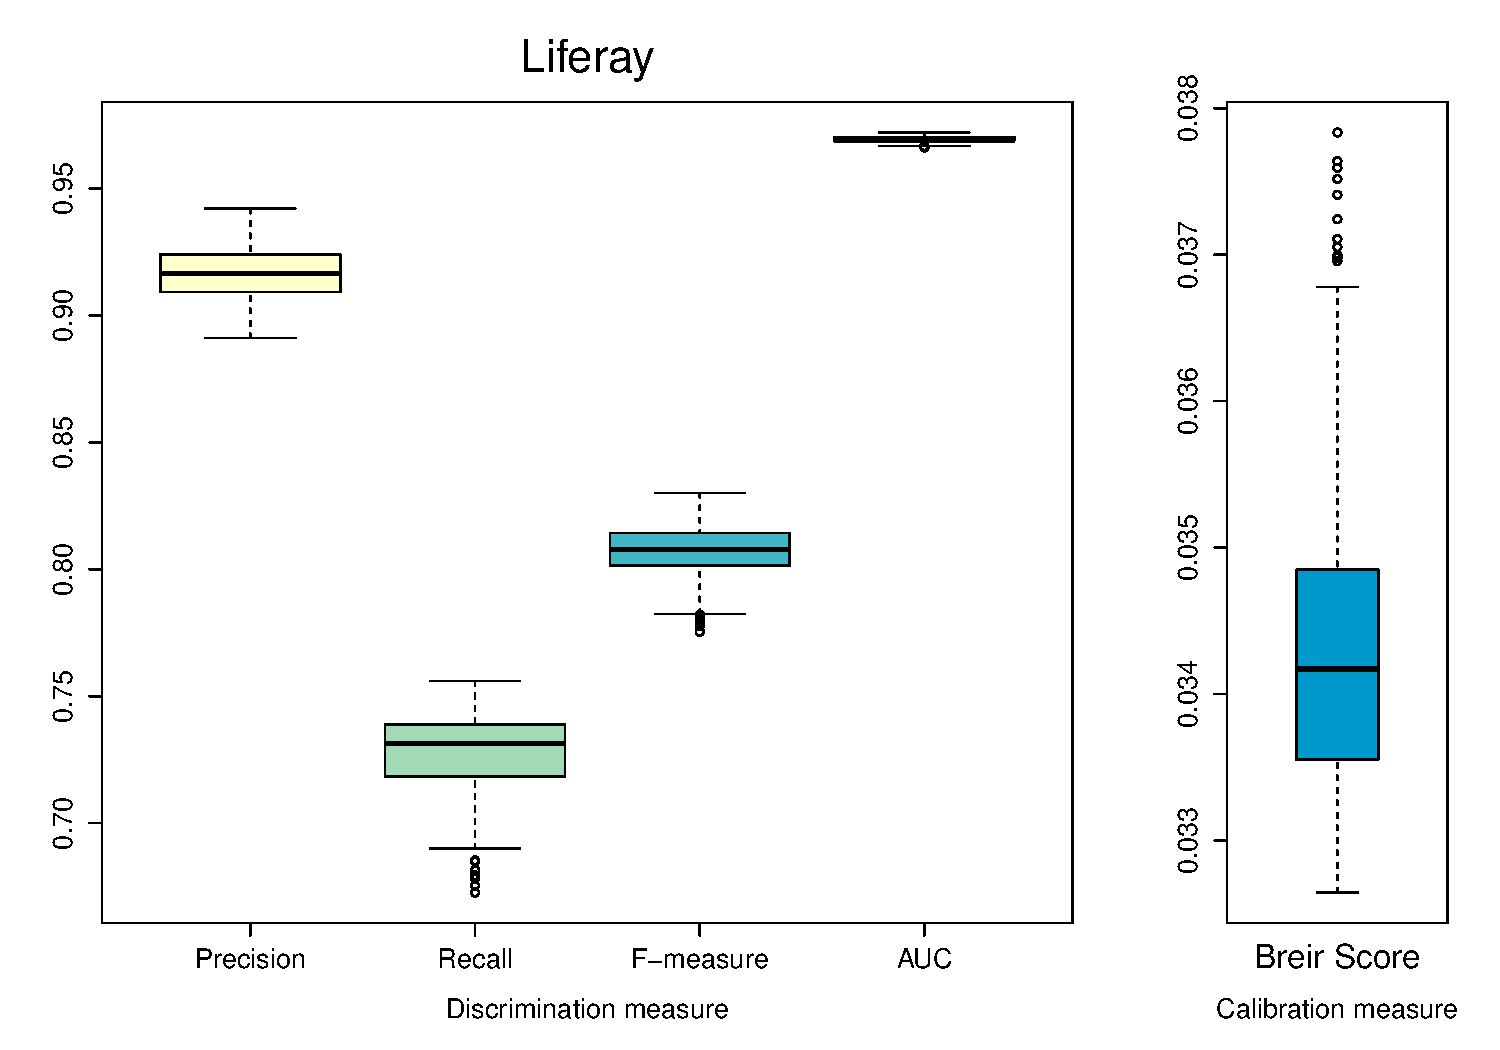
\includegraphics[width=0.69\columnwidth]{LRBox}\label{fig:f43}}
	\hfill
	%	\caption{Distribution of the number of developers responsible for changing a log}
	\caption{The optimism reduced performance measures of the four projects}
	\label{fig:optmisim}
	
\end{figure}

%\textbf{\noindent \textsl{(C4 - Importance of each metric in relation to log stability)}}
\subsection*{Step A2 - Identifying Important Metrics}

To find the importance of each metric in a random forest model, we use a permutation test. In this test, the model built using the bootstrap data (i.e., two thirds of the original data) is applied to the test data (i.e., remaining one third of the original data). Then, the values of the $X_{i}$ $^{th}$ metric of which we want to find importance for, are randomly permuted in the test dataset and the precision of the model is recomputed. The decrease in precision as a result of this permutation is averaged over all trees, and is used as a measure of the importance of metric $X_{i}$th in the random forest.





We use the \emph{importance} function defined in \emph{RandomForest} package of R, to calculate the importance of each metric. We call the \emph{importance} function every time during the bootstrapping process to obtain 1,000 importance scores for each metric in our dataset. 	



As we obtain 1,000 data sets for each metric because of bootstrapping process, we use the \textbf{Scott-Knott} (SK) clustering to group the metric based on their means~\cite{Cluster1,Cluster2}. This is done to group metrics which are important predictors for the likelihood of log change. The SK algorithm uses the hierarchical clustering approach to divide the metrics and uses the likelihood ratio test to judge the difference between the groups. This assures the means of metrics within a group not to be statistically significantly different. We use the \emph{SK}	 function in the \emph{ScottKnott} package of R and set the significance threshold parameter to 0.05 to cluster the metrics into different groups. 
%\begin{table}

%	\centering


\begin{table*}[t]
	\protect\protect\caption{The importance values of the metrics (top 10), divided into homogeneous
		groups by Scott-Knott clustering. The `+' and `-' signs signifing positive
		and negative correlation of the metric on log stability}
	
	\centering
	
	\begin{tabular}{lll|lll}
		\hline 
		& \textbf{ ActiveMQ}  &  &  & \textbf{Camel}  & \tabularnewline
		\hline 
		\textbf{Rank}  & \textbf{Factors}  & \textbf{Importance}  & \textbf{Rank}  & \textbf{Factors}  & \textbf{Importance} \tabularnewline
		\hline 
		1  & Developer experience  & 0.258 -  & 1  & Developer experience  & 0.297 - \tabularnewline
		2  & SLOC  & 0.188 +  & 2  & Ownership of file  & 0.161 - \tabularnewline
		3& Ownership of file   & 0.170 +  & 3 & Log level & 0.128  \tabularnewline
		4  & Log density  & 0.166 +  & 4  & SLOC  & 0.112 + \tabularnewline
		5  & Log variable count & 0.089 +  & 5 & Log density  & 0.108 - \tabularnewline
		6 & Log level & 0.078   &  & Type of log change & 0.106  \tabularnewline
		7  & Type of log change & 0.069   & 6  & Log variable count & 0.090 + \tabularnewline
		8  & Variable declared  & 0.055 -  & 7 & Old log & 0.071 - \tabularnewline
		9  & Log context & 0.043   & 9 & Log context & 0.061  \tabularnewline
		\hline 
	\end{tabular}
	
	\begin{tabular}{lll|lll}
		\hline 
		& \textbf{CloudStack}  &  &  & \textbf{Liferay}  & \tabularnewline
		\hline 
		\hline 
		\textbf{Rank}  & \textbf{Factors}  & \textbf{Importance}  & \textbf{Rank}  & \textbf{Factors}  & \textbf{Importance} \tabularnewline
		\hline 
		1  & Type of log change & 0.268   & 1  & SLOC  & 0.192 + \tabularnewline
		2  & Code churn in commit  & 0.243 +  & 2  & Developer experience  & 0.174 - \tabularnewline
		3& SLOC & 0.232 +  & 3 & Ownership of file  & 0.170 - \tabularnewline
		4  & Log density  & 0.208 -  & 4 & Log density & 0.158 - \tabularnewline
		5 & Ownership of file  & 0.154 -  & 5  & Log variable count  & 0.143 + \tabularnewline
		6 & Developer experience   & 0.119 +  & 6 & Variable declared  & 0.118 + \tabularnewline
		7  & Log text length  & 0.095 +  &7 & Log context  & 0.106  \tabularnewline
		8 & Log variable count  & 0.091 +  & 8  & Log text length & 0.071 + \tabularnewline
		9 & Variable declared  & 0.097 -  & 9  & Type of log change & 0.058 \tabularnewline
		\hline 
	\end{tabular} \label{tba:Scott} 
	
	
	
\end{table*}



%\label{tba:optmisim}
%\end{table}


\subsection{Results}

\hypobox{The random forest classifier achieves a precision of 0.89-0.91, recall of 0.71-0.83 and outperforms random guessing for our studied applications} 
Figure~\ref{fig:optmisim} shows the optimism-reduced values of \textsl{precision}, \emph{recall}, \emph{F-measure} and \emph{Brier score} for each project. The model achieves an AUC of 0.95-0.96 across the studied applications. The classifier achieves Brier scores between 0.04 and 0.07 across all projects. If the model achieves a Brier score of 0.07, it means our model can forecast with 73\% probability a log will change. Brier score reaches 0.25 for random guessing (i.e., predicted value is 50\%).
% We find the recall of the random forest classier in Liferay is not as high as the other projects. This may be because Liferay has the lowest total number of log lines and close to 50\% of the log changes are log relocations as seen in Table~\ref{tba:logtype}. Because of the lower percentage of logs which are changed, the random forest classifier has fewer nodes (trees) and likelihood of false negatives is higher. 

%lowest percentage of logs which are changed at 20\%, compared to 45-70\% in the other projects. Because of the lower percentage of logs which are changed, the random forest classifier has fewer nodes (trees) and likelihood of false negatives is higher. 

%\hypobox{The random forest classifier outperforms random guessing.} 

\begin{table}[tb]
	\centering
	\caption{Contribution of top 3 developers}
	
	\begin{tabular}{lrrr}		
		\cline{1-4} 	& Total logs & Changed logs & Total \# of contributors \\  \cline{1-4}
		ActiveMQ    & 956 (50.4\%)            & 301 (31.4\%)   & 41 \\
		Camel       & 3060 (63.1\%)              & 1460 (47.7\%) &   151	    \\
		Cloudstack  & 5982 (35.7\%)              & 2276 (38.0\%)  &  204  \\
		Liferay     &  3382 (86.7\%)            & 609 (18.0\%)     &  351 \\\cline{1-4}
		\textbf{Average}& \textbf{3345 (59\%)} & \textbf{1161} (\textbf{33.75\%})& 747 \\\cline{1-4}
		
	\end{tabular}
	\label{tba:topDevelopers}
\end{table}


\subsection*{{B2. Important metrics for log stability}}

%From Table~\ref{tba:Scott} we see that `file ownership', `SLOC', `log density', and `developer experience' are common across all the projects in our studied systems. 

%The high importance of \emph{SLOC}, \emph{code churn in commit} and \emph{\# of comments} indicate that log stability 

%% LyX 2.1.2 created this file.  For more info, see http://www.lyx.org/.
%% Do not edit unless you really know what you are doing.
\begin{figure}[tb]
	
	\centering
	\subfloat{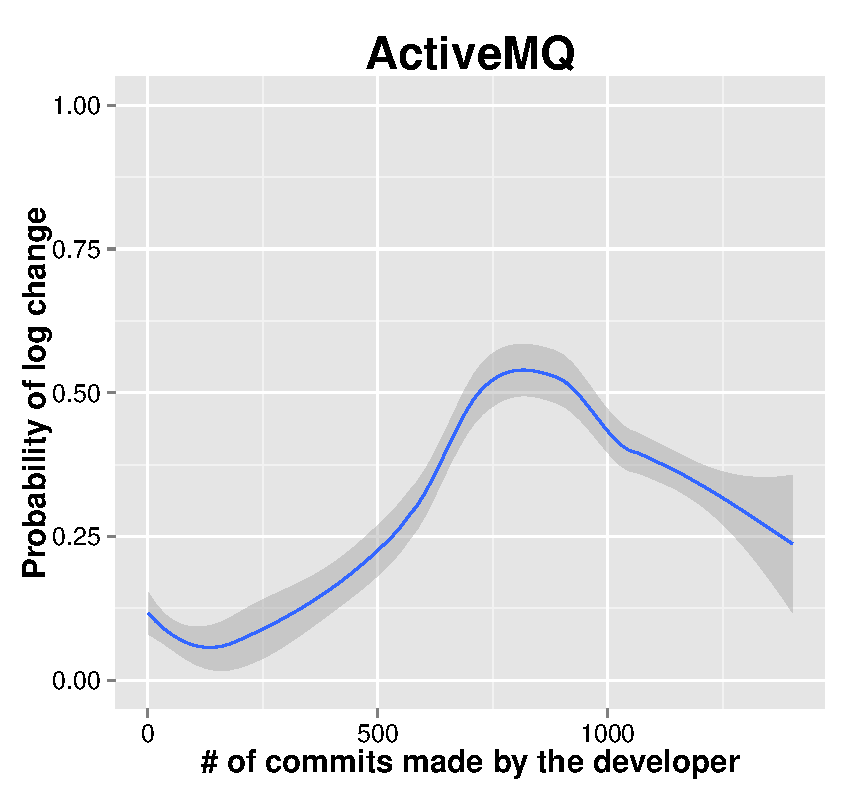
\includegraphics[width=0.49\columnwidth]{QP_Amq_Dxp}\label{fig:f4}}
	\hfill
	\centering
	\subfloat{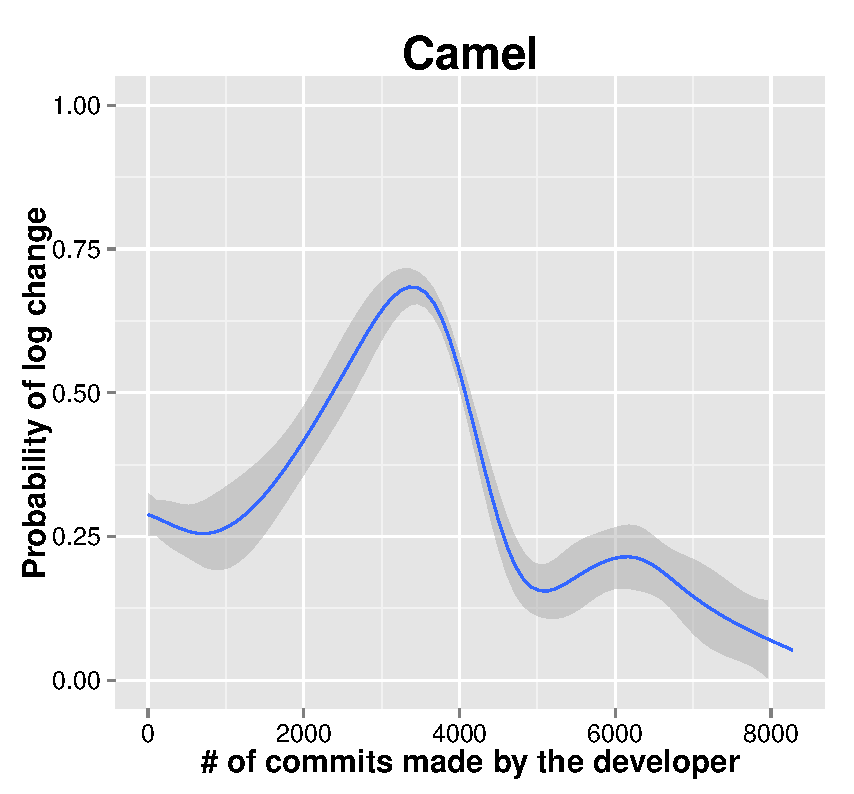
\includegraphics[width=0.49\columnwidth]{QP_Camel_Dxp} }
	\hfill
	\centering
	\subfloat{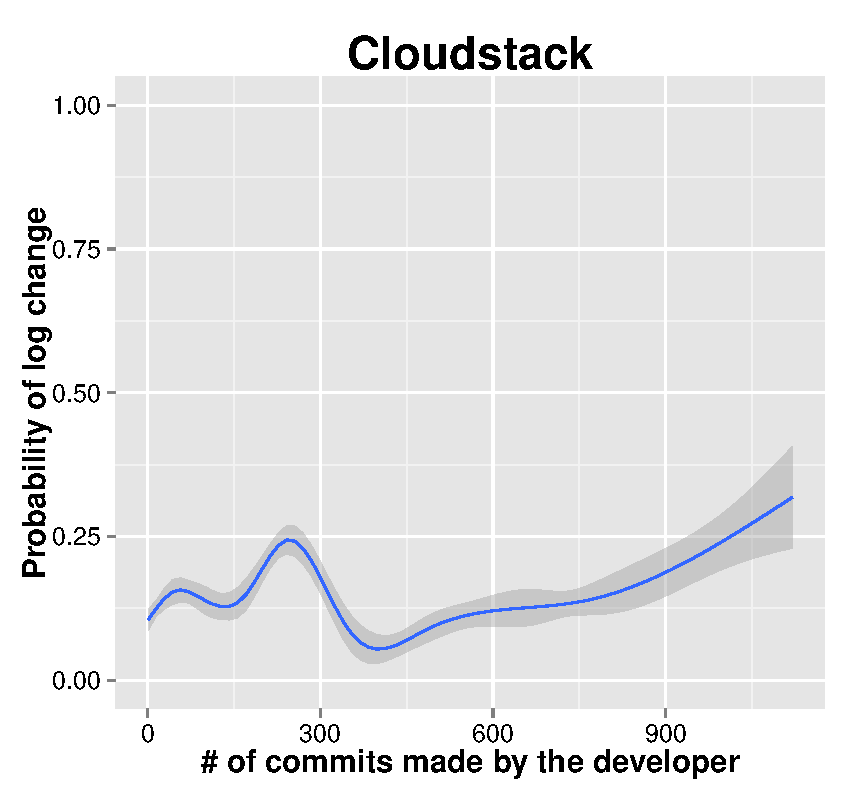
\includegraphics[width=0.49\columnwidth]{QP_Clo_Dxp}
		\label{fig:f4}}
	\hfill
	\centering
	\subfloat{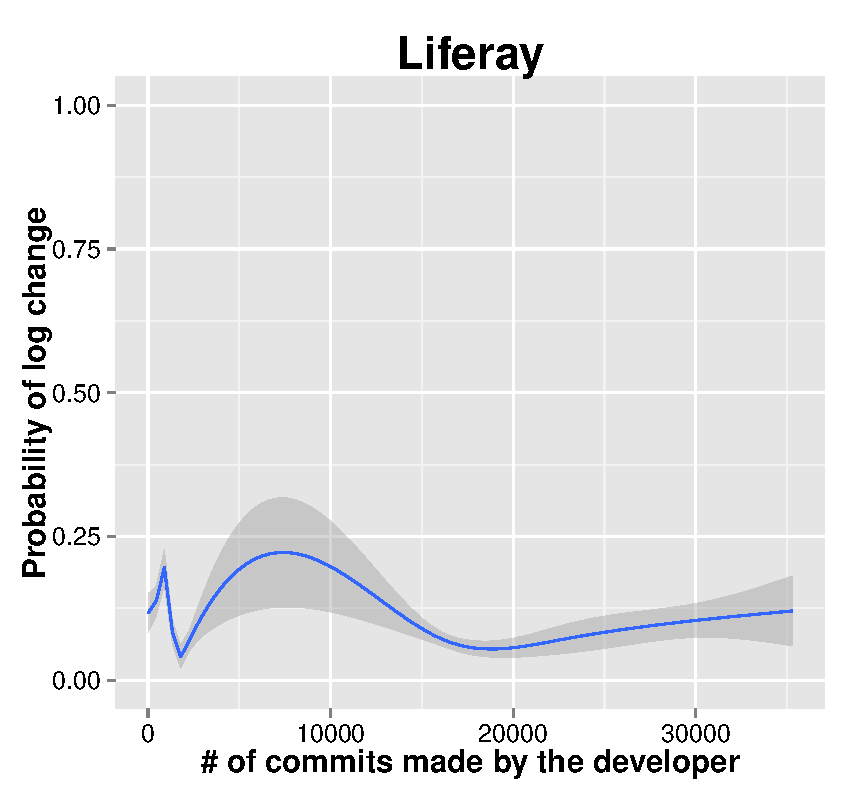
\includegraphics[width=0.49\columnwidth]{QP_Lif_Dxp}\label{fig:f4}}
	\hfill
	%	\caption{Distribution of the number of developers responsible for changing a log}
	\caption{Comparing experience of developers who add unchanged logs against logs changing more than once}
	\label{fig:Dexp_BP}
	
\end{figure}


%\begin{figure}[tb]
%	\centering
%	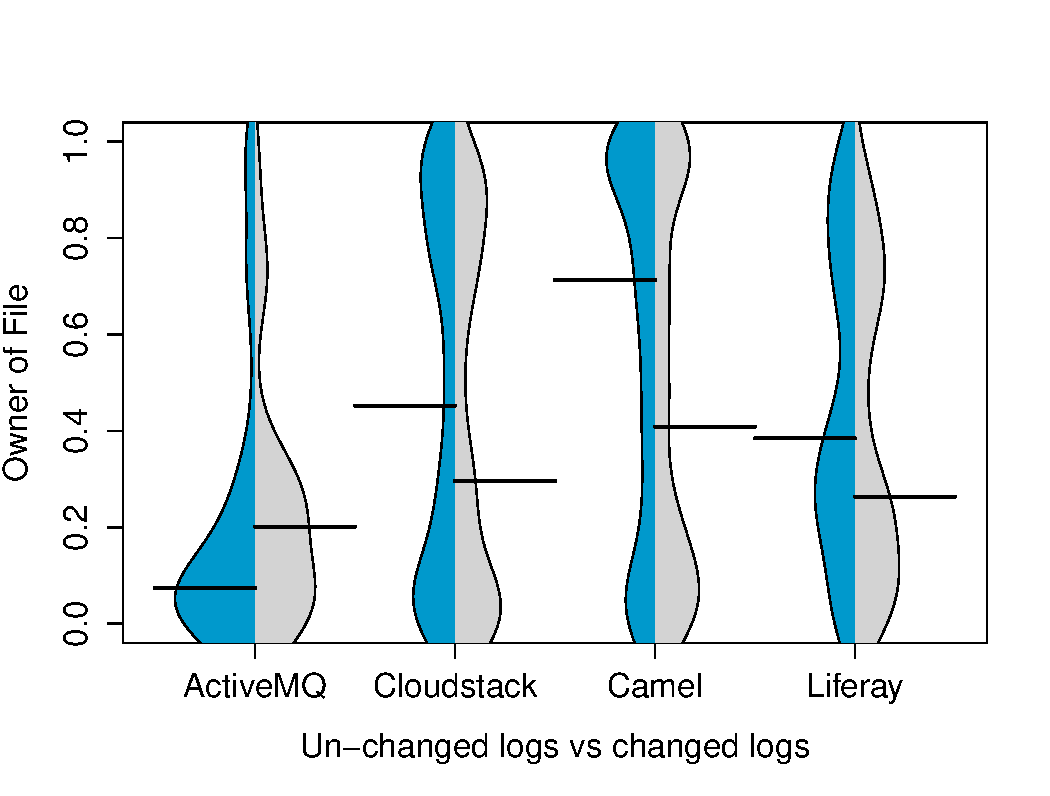
\includegraphics[width=1\linewidth]{ChangedvsUnchangedlogs}
%	\caption{Comparing the file ownership of developers who add logs that are never changed vs logs which are changed.}
%		\label{fig:ChangedvsUnchangedlogs}
%\end{figure}






\textbf{{{Developer experience} is an important metric to explain the likelihood of log change.}} From Table~\ref{tba:Scott}, we see that developer experience is one of top four metrics, to help explain the likelihood of a log being changed in all the studied applications. 
Figure~\ref{fig:Dexp_BP} shows the probabilities of a log being changed as developer experience increases, and it is interesting to note that in all the projects logs introduced by new developers have lower probability of being changed, when compared to more experienced developers. We also observe that as developers get more experience the probability of log change decreases in ActiveMQ, Camel and Liferay. This downward trend maybe be because in ActiveMQ, Camel and Liferay, the top three developers are responsible for adding more than 50\% of the logs as seen in Table~\ref{tba:topDevelopers}. We also find that only 30\% of the logs added by these top developers ever change. These findings, suggest that developers of log processing tools should be more cautious when using a log written by developers who have some experience in the application rather than new developers. 


%This suggests that logs which change are added by less experienced developers in ActiveMQ, Camel and Liferay. This can be seen in Figure~\ref{fig:Dexp_BP}, where logs which change three times or more are changed by less experienced developers, when compared to unchanged logs. For example, when we inspect \emph{git diff} for the file \emph{SessionBatchTransactionSynchronization.java} in Camel, we find that all the logs introduced by a new developer are fixed by a more experienced developer. In this case, the experienced developer changes the log contexts, i.e., relocates the logs and adds additional context information to provide more meaning to the logs. 


%We also find that in ActiveMQ, Camel and Liferay, the top three developers are responsible for more than 50\% of the logs. Only 30\% of the logs added by these developers are changed as seen in Table~\ref{tba:topDevelopers}. This result recommend that new developers should get more experience about the application by actively making more commits to write more stable logs. 

\begin{figure}[tb]
	
	\centering
	\subfloat{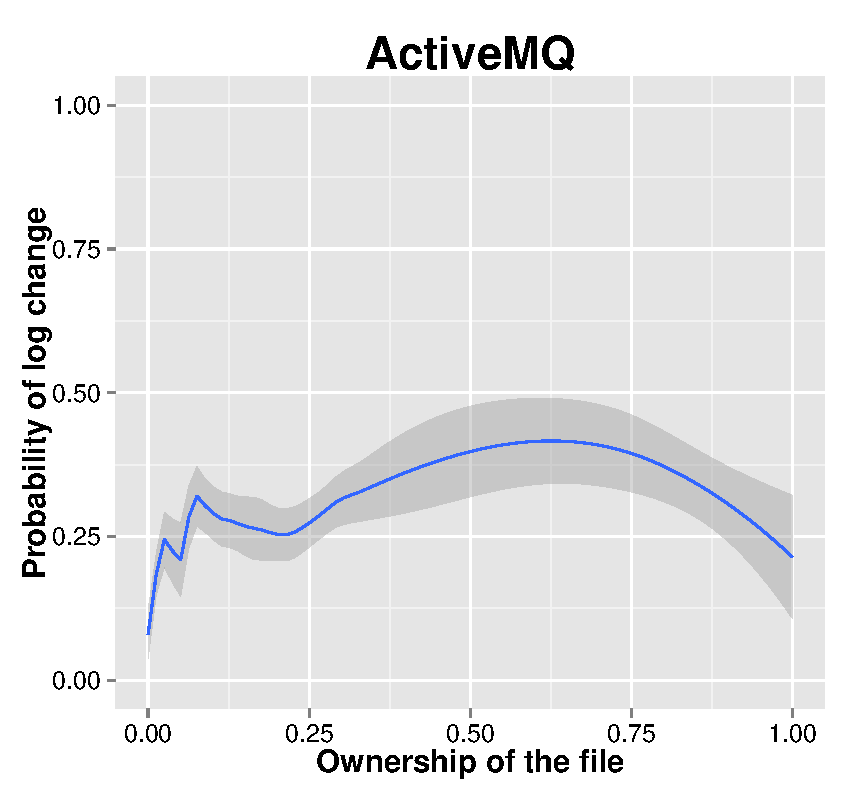
\includegraphics[width=0.49\columnwidth]{QP_Amq_Ow}\label{fig:f4}}
	\hfill
	\centering
	\subfloat{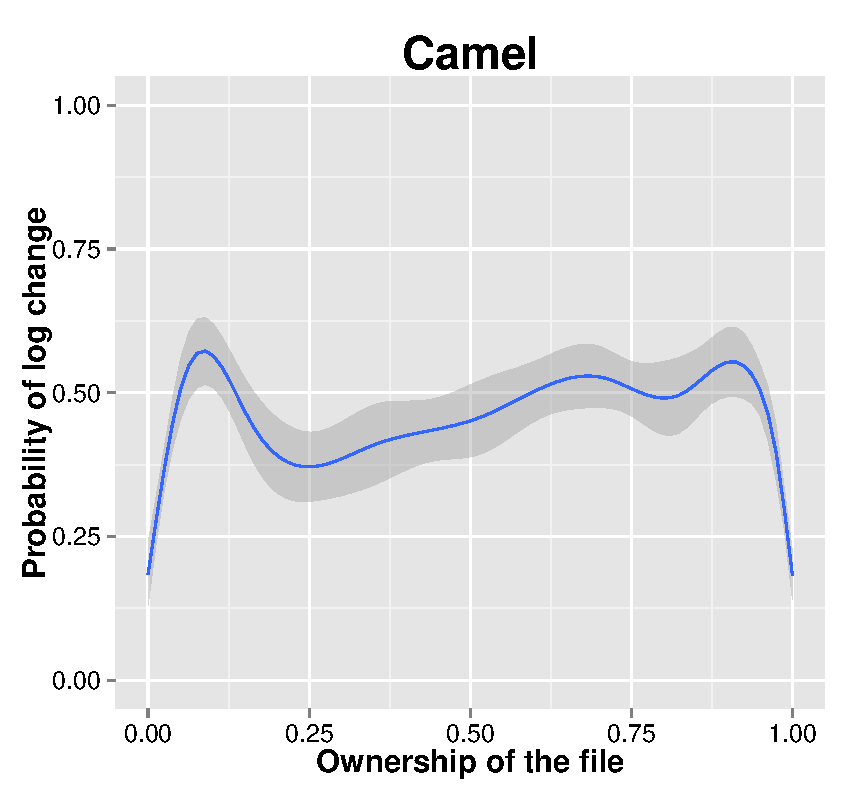
\includegraphics[width=0.49\columnwidth]{QP_Camel_Ow} }
	\hfill
	\centering
	\subfloat{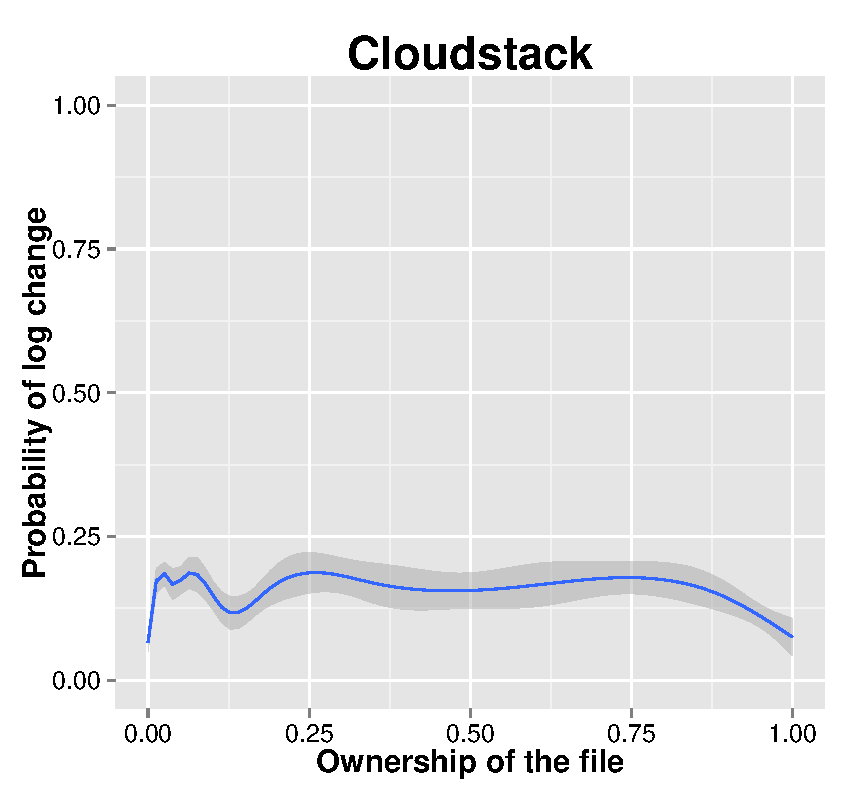
\includegraphics[width=0.49\columnwidth]{QP_Clo_Ow}
		\label{fig:f4}}
	\hfill
	\centering
	\subfloat{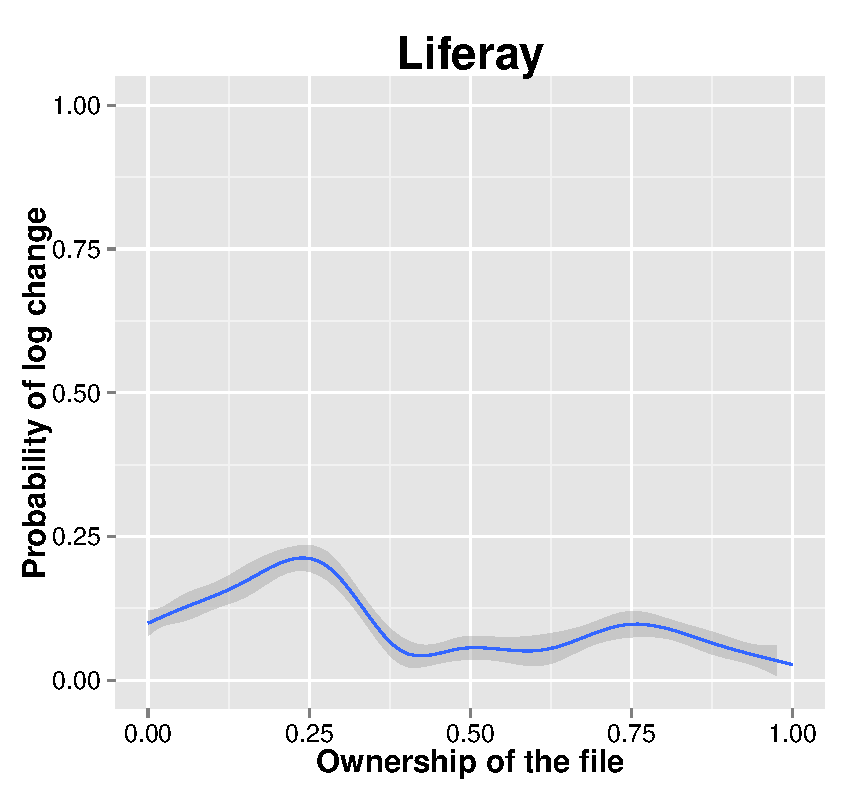
\includegraphics[width=0.49\columnwidth]{QP_Lif_Ow}\label{fig:f4}}
	\hfill
	%	\caption{Distribution of the number of developers responsible for changing a log}
	\caption{Comparing file ownership of developers who add unchanged logs against logs changing more than once}
	\label{fig:Numberofchanges_BP}
	
\end{figure}

%\begin{table}[tb]
%	\centering
%	\caption{Contribution of developers having less than 25\% ownership in a file}
%	
%	\begin{tabular}{lrrr}		
%		\cline{1-4} 	& Total logs & Changed logs &  \\  \cline{1-4}
%		ActiveMQ    & 1402 (73.9\%)            & 400 (28.5\%)   & 41 \\
%		Camel       & 3060 (63.1\%)              & 1460 (47.7\%) &   151	    \\
%		Cloudstack  & 5982 (35.7\%)              & 2276 (38.0\%)  &  204  \\
%		Liferay     &  3382 (86.7\%)            & 609 (18.0\%)     &  351 \\\cline{1-4}
%		\textbf{Average}& \textbf{3345 (59\%)} & \textbf{1161} (\textbf{33.75\%})& 747 \\\cline{1-4}
%		
%	\end{tabular}
%	\label{tba:bottomOwnership}
%\end{table}



\textbf{{Ownership of the file is an important metric to explain the likelihood of log change.}} From Table~\ref{tba:Scott}, we see that ownership of the file is one of top four metrics after developer experience to help explain the likelihood of a log being changed in all the studied applications. From Figure~\ref{fig:Numberofchanges_BP}, we observe that in all the applications that logs introduced by developers who own more than 75\% of the file are less likely to be changed. We also observe that developers who own less than 20\% of the file are responsible for 27\%-67\% of the log changes in the studied applications, which is seen as upward trend from 0 to 0.20 in Figure~\ref{fig:Numberofchanges_BP}. These results suggest that developers of log processing tools should be more cautious when using a log written by developers who have contributed to less than 20\% of the file in the studied applications.

 

% and logs introduced by developers who own less than 25\% are more likely to be changed. 
%
%\begin{figure}[tb]
%	
%	\centering
%%	\subfloat{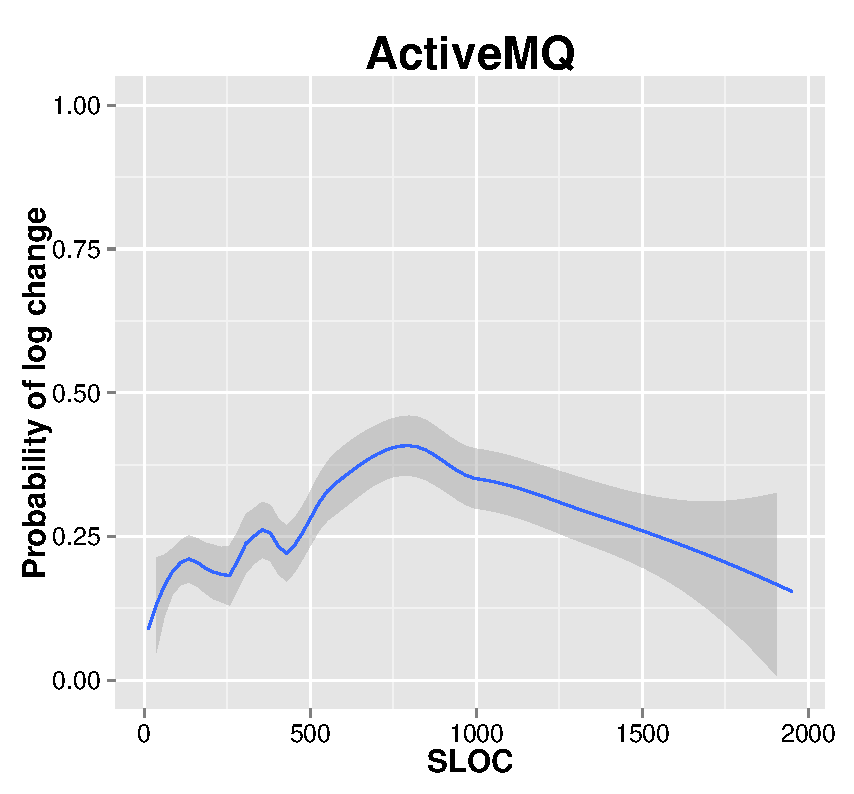
\includegraphics[width=0.49\columnwidth]{QP_Amq_SLOC}\label{fig:f4}}
%	\subfloat{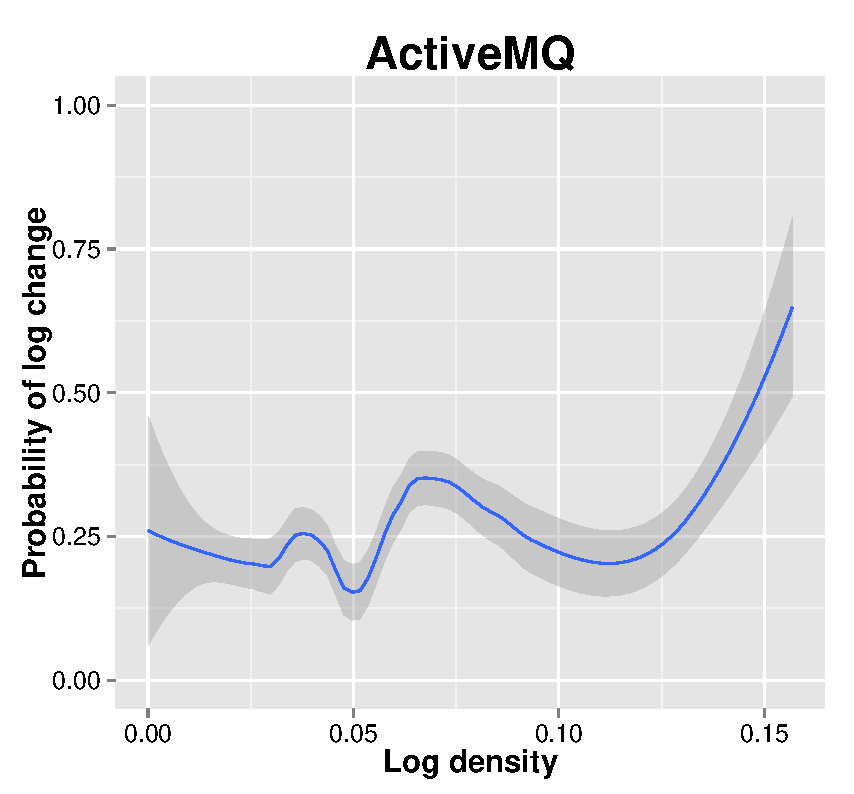
\includegraphics[width=0.49\columnwidth]{QP_Amq_Ld}\label{fig:f4}}
%	\hfill
%	\centering
%%	\subfloat{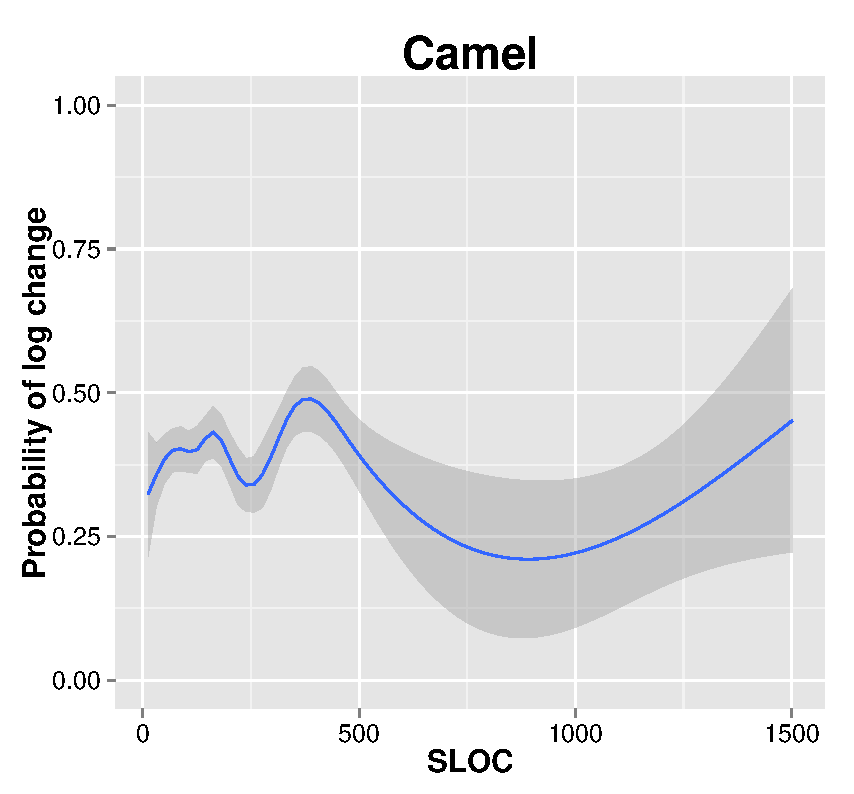
\includegraphics[width=0.49\columnwidth]{QP_Camel_SLOC} }
%		\subfloat{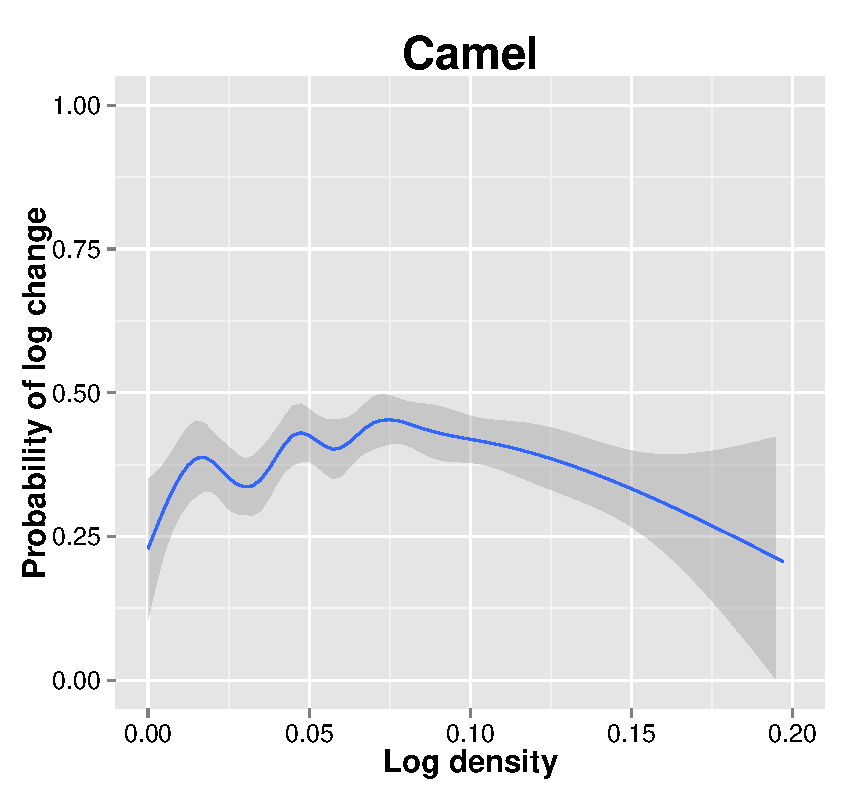
\includegraphics[width=0.49\columnwidth]{QP_Camel_Ld}\label{fig:f4}}
%	\hfill
%	\centering
%%	\subfloat{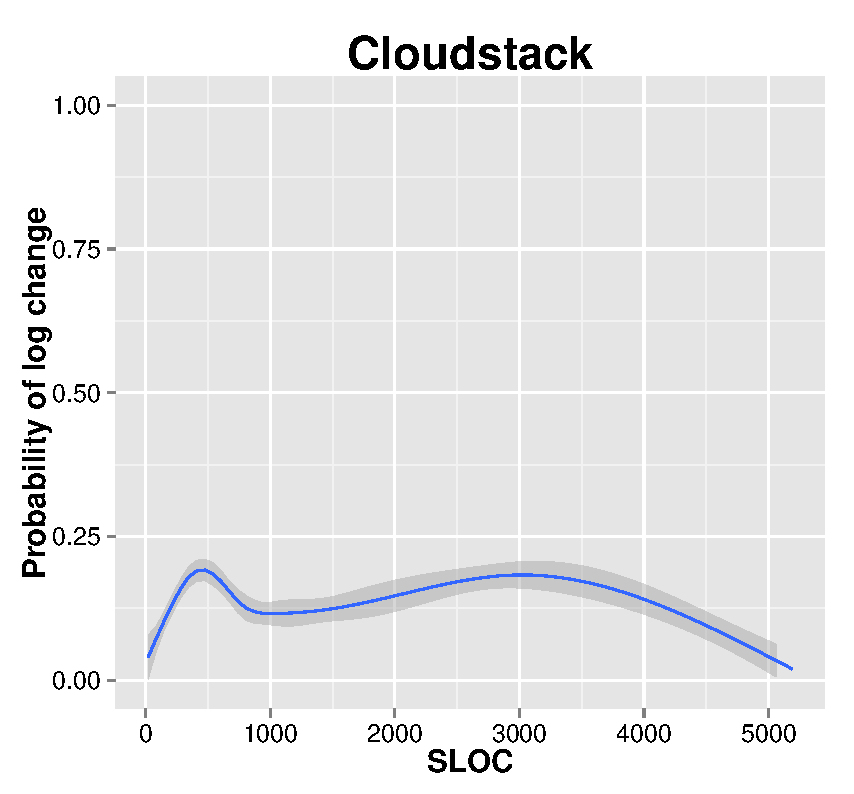
\includegraphics[width=0.49\columnwidth]{QP_Clo_SLOC}}
%			\subfloat{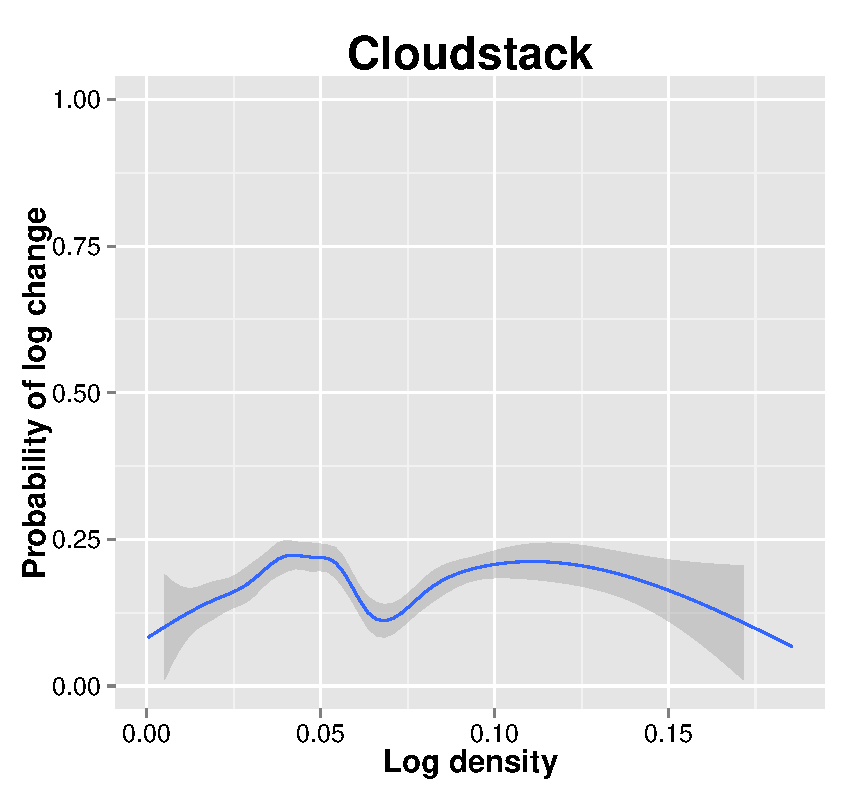
\includegraphics[width=0.49\columnwidth]{QP_Clo_Ld}\label{fig:f4}}
%%
%	\hfill
%	\centering
%%	\subfloat{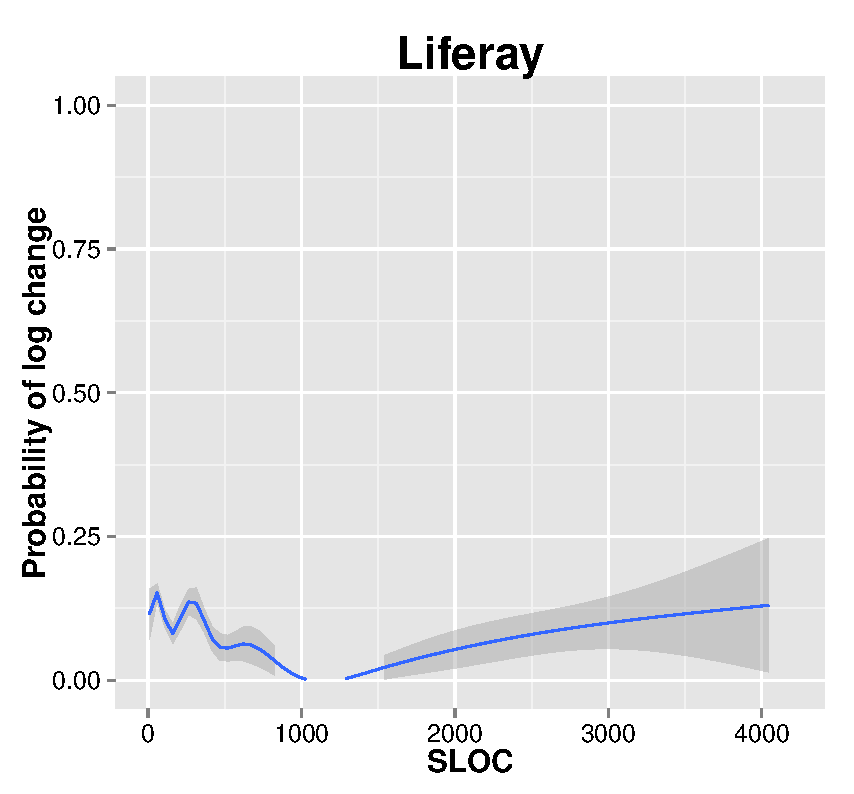
\includegraphics[width=0.49\columnwidth]{QP_Lif_SLOC}\label{fig:f4}}
%		\subfloat{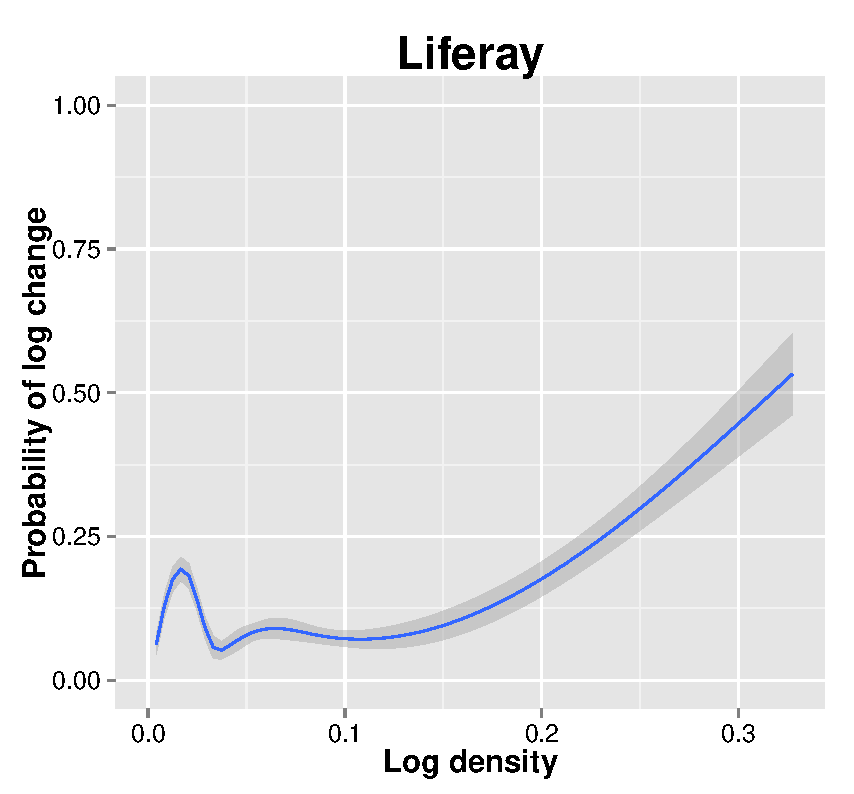
\includegraphics[width=0.49\columnwidth]{QP_Lif_Ld}\label{fig:f4}}
%	\hfill
%	%	\caption{Distribution of the number of developers responsible for changing a log}
%	\caption{Comparing file ownership of developers who add unchanged logs against logs changing more than once}
%	\label{fig:LD}
%	
%\end{figure}
%


%  suggests that logs added by developers who have little ownership are more unstable and more likely to be changed. This is show by Figure~\ref{fig:Numberofchanges_BP}, where in Camel and Liferay, the unchanged logs are introduced by developers who have more ownership of the file. We also find that the most unstable logs i.e., (3 + changes ) in Camel, Cloudstack and Liferay are done by developers who have lesser ownership of the file, accounting for the negative correlation in these three applications. These results suggest that developers who are not owners of a file, should be more cautious	 when adding or changing logs in the file. For example when we inspect the \emph{git diff} for the file \emph{SSLContextServerParameters.java} in Camel, we find that the owner of the file fixes the changes made by a non-owner by increasing the logging level to reduce a flood of logs being generated. 


%This is seen in Figure~\ref{fig:ChangedvsUnchangedlogs}, where in Camel and Liferay, the logs which change are more likely to be added by developers who have less ownership on the files, than logs which are never changed. We also find that when logs change, the developers making the changes have less ownership than developers adding the log. From Figure~\ref{fig:Numberofchanges_BP} we see that in Camel, Cloudstack and Liferay, the logs which change more than three times are done by developers who have lesser ownership of the file, accounting for the negative correlation in these applications. These results suggest that developers who are not owners of a file, should be more cautions when adding or changing logs in the file. For example when we inspect the \emph{git diff} for the file \emph{SSLContextServerParameters.java} in Camel, we find that the owner of the file fixes the changes made by a non-owner by increasing the logging level to reduce a flood of logs being generated. 

%when logs are changed by developer who has less ownership, an experienced developer reverts fixes the same logs again. 


% where we find that in Camel, Cloudstack and Liferay unchanged logs are introduced by developer who have higher ownership than developers introducing changed logs. 

%After identifying the frequency of changes within the studied applications, we find the number of the developers responsible for the log changes and also if they own the file which contains the log. We use the developer name available from the `git log' to count the number of developers who change a log. To decide whether a developer owns a file we calculate the ratio of number of lines written by him to the total lines of code using the `blame' command available in Git. Since \emph{blame} only shows the changes made to a file in the last commit, to calculate the contribution of a developer to a file we recursively look at changes made in previous commits by that developer. We use the \emph{blame} to calculate the contribution at each commit and take the mean contribution across all commits to find his ownership of a file.



% which implies a) logs introduced by more experienced developers are more likely to change or b) experienced developer introduce more logs in the studied application.

%We find that the top 3 developers introduce 59\% of the total logs in the studied applications as seen in Table\ref{tba:topDevelopers}. We also find that close to 64\% of the logs which change are from these experienced developers. This results suggest that even though experienced developers introduce majority of logs, they is no increase in log stability. 



%where in three of the studied applications, the logs which change are introduced by developers who have lower ownership of a file. 



%which are changed as seen in Table~\ref{tba:topDevelopers}. This suggests that even though 

%Even though ActiveMQ and Liferay has positive correlation in Table~\ref{tba:Scott}, we find that these projects have strong code ownership and  two developer are responsible for over 50\% of the total commits within the projects. To remove this strong ownership, we exclude the log changes made by these top developers in ActiveMQ and Liferay and we find that developer experience has negative correlation in both ActiveMQ and Liferay. This suggests that logs which are introduced by more experienced developers are less likely to change in all of the studied applications. 


%
\textbf{{{Log density} is an important metric in our studied applications to explain the likelihood of log change.}} From Table~\ref{tba:Scott}, we see observe that log density has the highest importance in Liferay and Cloudstack. We find that in these two applications, the logs which change are present in files with lower log density than unchanged logs. When we measure the median file sizes we find that, logs which change more are present in files with significantly higher SLOC (2x-3x higher). This suggests that large files which are not well logged are more likely to have unstable logs, than well logged files.



%From Figure~\ref{fig:LD} we see that increase in log density increases the likelihood of log change in ActiveMQ and Liferay. In these systems, we find that the files with highest log densities have significantly lower SLOC (10x smaller) than the median, implying that too many logs can decrease code readability 

% and decreases the likelihood of log change in Cloudstack and Camel. When we measure the median file sizes for Cloudstack and Camel, we find that logs which change more are present in files with significantly higher SLOC (2x-3x higher). 



%We find that log density has negative correlation with log stability (i.e., increase in log density decreases probability of log change), in Camel, Cloudstack and Liferay as seen in Table~\ref{tba:Scott}. We find that in these applications, the logs which change are present in files with lower log density than unchanged logs. When we measure the median file sizes we find that, logs which change more are present in files with significantly higher SLOC (2x-3x higher). T 
 
%have significanlty 

%more than three times are present in files with low density i.e., not a well logged file but more SLOC than files with unchanged logs.

 
% the log density for logs changing 1-2 times is higher than unchanged logs, but w


%{{log variable count} has a positive correlation with log stability as shown in Table~\ref{tba:Scott}.}
%This implies that more variables in a log results in a higher likelihood that a log will be changed. This may be because there are inconsistencies between logs and the actual needed information intended as shown by prior research~\cite{Characterizinglogs} and developers have to update logs to resolve the inconsistencies. We find that the median for changed logs in all the subject systems is two variables for 


%\textbf{We find that \emph{SLOC}(source lines of code) is a strong predictor of log change across all projects.} \emph{SLOC} has a positive correlation suggesting that logs in larger files have higher a likelihood of getting changed. 

%We find that \emph{Variable declared} has positive correlation in three of the studied systems, which suggests that when developers add new variables in the commit there is a higher likelihood of log change as they may add or modify the log to output the new data.
%, logs around those comments are less likely to get changed. 


% is also a strong predictor of log change in all our models but the correlation is split within the projects. We find that in Cloudstack and Camel, developer experience has a negative correlation on log change, where as in ActiveMQ and Liferay developer experience has positive correlation. 
%The positive correlation may be because of strong code ownership seen ActiveMQ and liferay where two developer are responsible for over 50\% of the total commits within the projects. To remove this strong ownership, we exclude the log changes made by these top developers in ActiveMQ and Liferay and we find that developer experience has positive correlation in ActiveMQ. This suggests that logs which are introduced by more experienced developers are less likely to change in three of the studied systems. 

 

%We find that positive correlation might be due strong code ownership in ActiveMQ and Liferay where two developers are responsible for over 50\% of the total commits, within these projects. The negative effect in ActiveMQ and Cloudstack suggests that logs written by more experienced developers are less likely to be changed. 



% This suggests that either (1) more experienced developers have logged the file increasing the stability of the logs or (2) less experienced developers have logged the file making logs unstable. 
%
%In these systems we find that, more logs are introduced by developers with less experience than developers greater experience. 


%This may be because (1) logs that are added by less experience developers are less stable or (2) more experienced developers might not be as careful about logging as new developers.

 

%
% This implies that logs introduced by more experienced developers and are more likely to be changed.  This may be because the experienced developers may be more complacent than less experienced developers, who thoroughly log the code. 

%We find that other metrics from the developer dimension are not consistent among the studied systems. This may be because each project might have different philosophy of development, for example we find that \emph{resolution time} has negative effect in Liferay and Camel but has positive effect in ActiveMQ. This suggests that logs are more likely to change in ActiveMQ when the resolution time of issue increases, but less likely in Liferay and Camel. 


\hypobox {Our Random Forest classifier achieves a precision of 89\%-91\% and recall of 71\%-83\% across all studied applications. We find file ownership, SLOC, developer experience and log density to be important predictors of log change in our studied applications.}






